\chapter{Implementation}

The camera calibration will be implemented using Python and the OpenCV library that offers all necessary functionality to fulfill the task.

A step-by-step documentation is provided by the developers of OpenCV \cite{cv_cctut}, which will be used as guidance in the following process.

Before the implementation can start, the necessary video material files \texttt{chessboard\_000.h264} and \texttt{chessboard\_019.h264} need to be downloaded and saved. In the following, they will be called video 1 and video 2, respectively.

Video 1 if focusing on showing the chessboard closer to the camera, but therefore also at the outer edge of the image to capture the fisheye effect of the camera.

Video 2 focuses on showing the chessboard in a bigger distance so the distortion effect can also be captured for objects further away in the threedimensional room.

\section{Extracting video frames}
Having set up the development environment, first the individual frames of the videos need to be extracted to be able to process them in the following steps.

For this, a class \texttt{VideoFrameExtractor} has been created. It wraps the OpenCV class \texttt{VideoCapture}, responsible for video handling, so it can be used more easily. \cite{cv_videocapture}

As a constructor argument, it accepts the filename of the video file. This filename will be provided to the OpenCV class to create a new \texttt{VideoCapture} object.

First, the wrapper offers a method \texttt{get\_frame\_count()} which returns the amount of frames the given video has. It uses the \texttt{get()} method of the object using the flag \texttt{CAP\_PROP\_FRAME\_COUNT} as parameter to retrieve the frame count from the video metadata.

Sadly, this method returns a negative value for the given videos. The reason is that they are provided as video streams - so while being encoded with the compatible H264 codec, they don't offer time information in the metadata (e.g. video length). The OpenCV method then cannot determine the frame count directly.

To workaround this issue, a fallback mechanism can be used, which simply loops through all frames of the video using the \texttt{read()} method and increments a counter for each of them. When the end of the video is reached, the counter value will be returned as the frame count.

This workaround is time- and calculation intensive however, especially when this process has to be repeated. So instead of using the provided videos directly, they first have been converted to regular MP4 files with timestamps. This has been done using the open source software \enquote{ffmpeg} using the parameters \texttt{-i input.h264 -c copy output.mp4}. It quickly fixes the file to conform to the regular MP4 file format, including all necessary metadata, without having to re-encode the video. This means the picture quality will not decrease since the existing frames are reused directly.

Using both methods, it can be determined that video 1 has 1801 frames while video 2 has 899 frames.

Moreover, the wrapper has two method to get the actual frames from the video. The first one \texttt{get\_video\_frames(frame\_ids)} returns only the frames with the IDs requested using the parameter. Similar to the frame count method, it loops through all frames of the video and adds the frame to a list, if the current frame ID can be found in the provided parameter list. To speed up the process, instead of looping through all frames, it is possible to always seek to the next requested frame, skipping all others.

The OpenCV method \texttt{set(cv.CAP\_PROP\_POS\_FRAMES, frame\_id)} is capable of doing that, which sets the next frame to be returned with the \texttt{read()} method. This method also relies on correct video metadata, so it can only be used with the reprocessed video.

The second method \texttt{get\_video\_frames\_generator()} returns all the frames of the video - necessary for detecting the chessboard in every single frame. This method could be realized similarly to the first method with a loop  that adds a frame to a list in each iteration.  This would use a big amount of memory however, since every single frame would be stored uncompressed in the list. Even for the short videos provided, this filled up more than 2 GB of memory.

\begin{lstlisting}[caption={Getting frames of the video using \texttt{yield}}, label={lst:yieldframe}]
def get_video_frames_generator(self):
    cap = cv.VideoCapture(self.filename)
    try:
        while cap.isOpened():
            ret, frame = cap.read()
            if not ret:
                break
            yield frame
    finally:
        cap.release()
\end{lstlisting}

To solve this issue, a \emph{generator} is used. Instead of returning the complete list of frames, an iterator is returned that returns the frames on-demand \enquote{lazily}, when the caller of the function actually iterates over the \enquote{list} (iterator). \cite{python_generator} The user of the function doesn't notice this directly since it behaves as if iterating over a list.

Python offers easy support for this using the \texttt{yield} keyword, which can be used instead instead of adding each frame to a list. The implementation can be found in \autoref{lst:yieldframe}. Using this implementation, only one frame at a time is in memory, significantly reducing memory usage.

\section{Finding frames with a detectable chessboard}
Now having the implementation for getting the frames from the videos, the chessboard has to be detected on them.

OpenCV offers the \texttt{findChessboardCorners()} function which can detect a chessboard on a single image. It needs an image and the size of the chessboard to be searched for as parameters. \cite{cv_cctut} The size of the chessboard is determined by the amount of rows and columns of internal corners. In the given videos, the chessboard has 8x8 squares, resulting in 7x7 internal corners.

Additionally, flags can be provided to the function. The two major flag options are to use adaptive thresholding to convert the image to black and white, and/or to only run a fast check so the function returns more quickly in case no chessboard is detected.

To save computation time, instead of detecting the chessboard on every program run from scratch, the detection can be done once and the IDs of the frames that had a detection can be saved. This way, it is not necessary to loop through all frames again for the following steps. Saving the IDs also doesn't take up much disk space, unlike the individual frames.

\begin{lstlisting}[caption={Detecting chessboards}, label={lst:chessboard_detect}]
def detect_chessboard_frame_ids(self) -> List[int]:
    found_ids = []
    for frame_id, frame in enumerate(self.frames):
        gray = cv.cvtColor(frame, cv.COLOR_BGR2GRAY)
        ret, _ = cv.findChessboardCorners(gray, self.ch_size, cv.CALIB_CB_FAST_CHECK)
        if ret:
            found_ids.append(frame_id)
    return found_ids
\end{lstlisting}

For this, a method \texttt{detect\_chessboard\_frame\_ids()} has been created, that loops through the frames of a video provided by the \texttt{VideoFrameExtractor} class and performs a quick detection using the \texttt{CALIB\_CB\_FAST\_CHECK} flag of the OpenCV function. On a detection, the frame ID is saved in a list, which is then finally returned. This implementation can be seen in \autoref{lst:chessboard_detect}. This list then can be printed on the console and its output then copied into the source code, so the frame IDs with detections are saved persistently.

When running the mentioned approach on both videos with 7x7 internal corners to be found, the results were not promising however. In video 1, only 10 frames with chessboard were detected; in video 2 even zero frames. These are detection rates significantly smaller than 1 \%.

To the human eye, there are many more frames where the full chessboard can be seen in the videos however - but the OpenCV function can't detect them. As the used algorithm is complex, it is not possible to pinpoint a specific reason. One possible cause is that the person holding the chessboard is partially obstructing the outermost squares with his fingers. Additionally, the OpenCV documentation states the chessboard used should have a big white border to improve detection, while the used chessboard is borderless. \cite{cv_cctut}

Since the videos with the chessboard used are not changeable because of the task exercise, one different possibility to improve the detection rate is to reduce the size of the chessboard to be detected by OpenCV. It should only be reduced as little as possible though because this can reduce the accuracy of the results. A 3x3 chessboard may be detected easily in a actual-7x7-chessboard, but it could be randomly detected somewhere in the chessboard frame - in the center, on the right, on the top left, ...; as can be seen in \autoref{fig:redviz}. Each of them has a different distortion depending on the position in the image.

\begin{figure}[h]
    \centering
    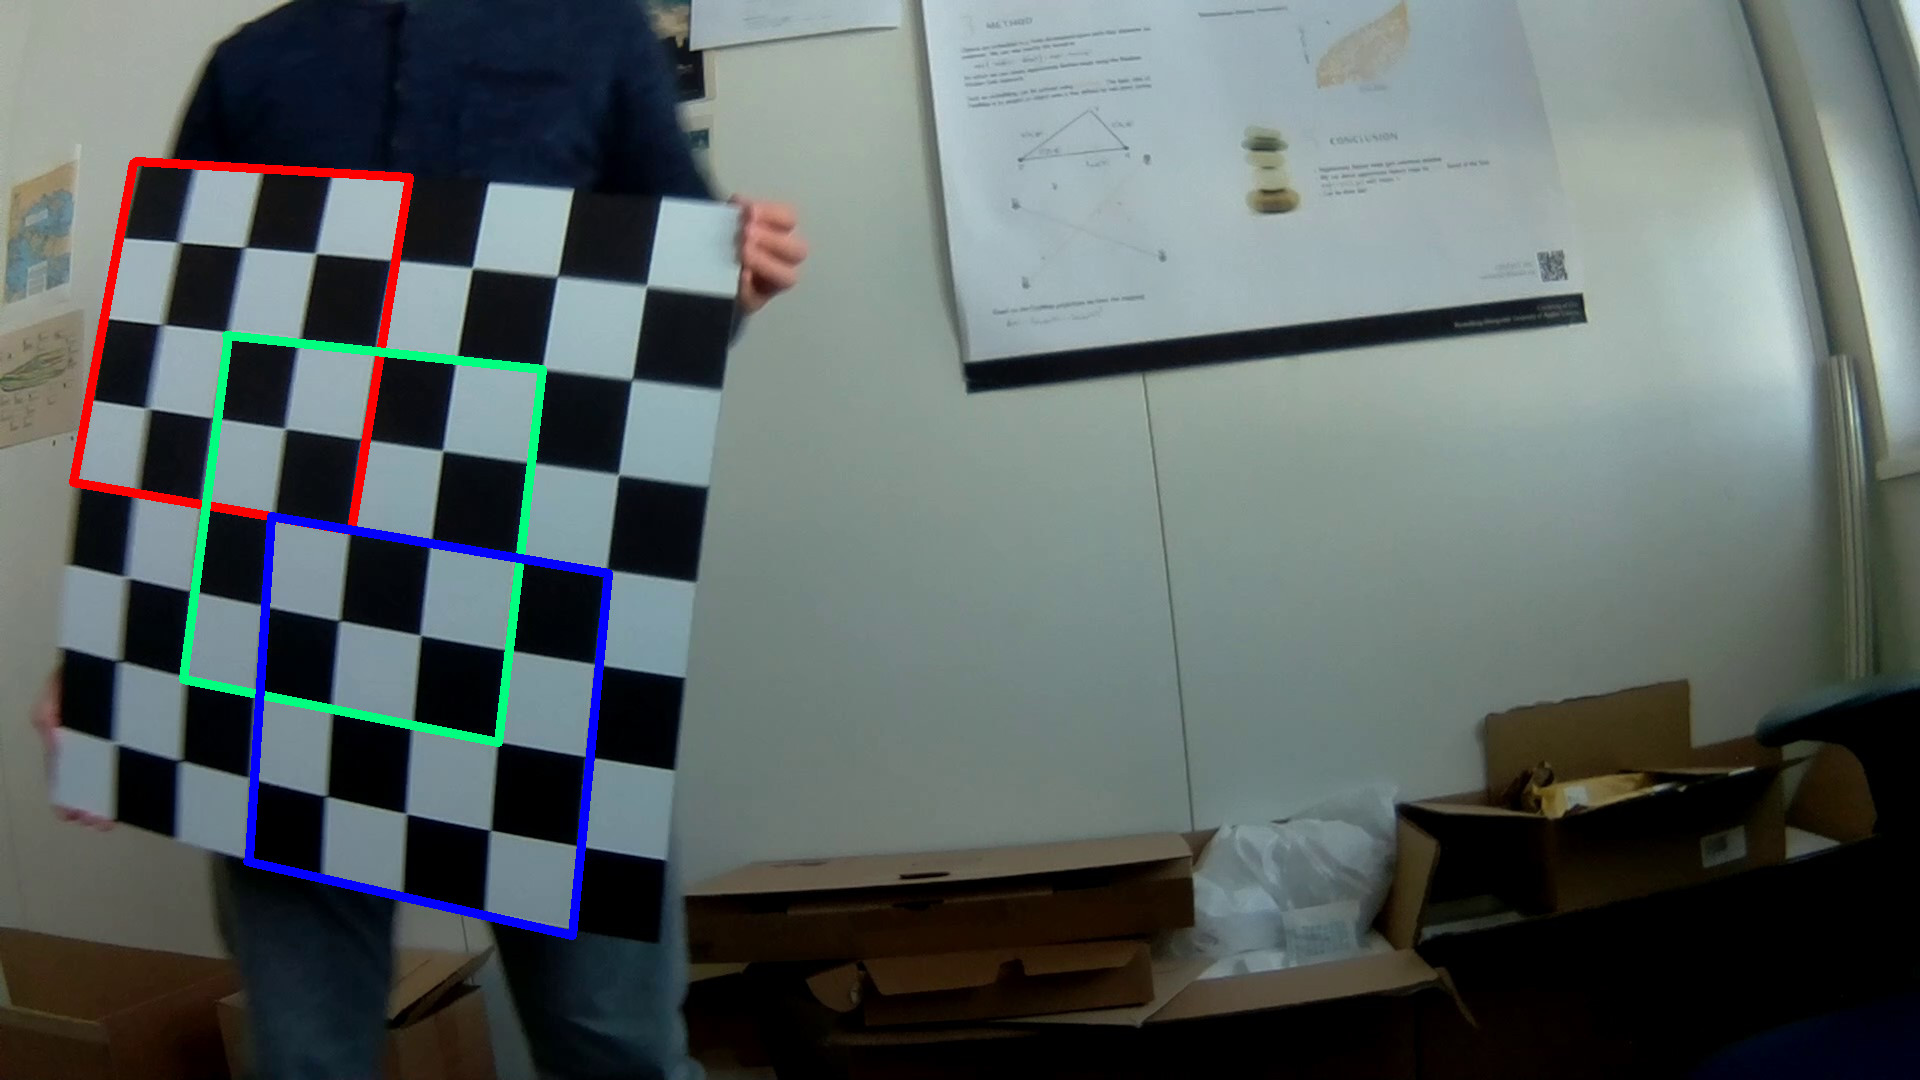
\includegraphics[width=0.8\textwidth]{figures/red_viz.jpg}
    \caption{Multiple possible 3x3 detections in 7x7 chessboard}
    \label{fig:redviz}
\end{figure}


That's why as a first step, the chessboard size to be found has been reduced to 7x6 and 6x7. The order of rows and columns in practice doesn't matter for this step, because in both cases the same 108 frames have been detected in video 1 and the same 21 frames in video 2 (respectively 6 \% and 2 \% of all frames).

While this is a better result than with 7x7, the detection rate is still low, especially in video 2. One possible cause is that the video has been shot with background light from the windows, which forced the camera to change its exposure and brightness when the person moved in the background. The already small, hard to detect chessboard now got underexposed additionally, making a corner detection more difficult because of the weak gradient between the black and (now) grey squares of the chessboard.

To solve the exposure problem, either a well-lit room without changing light conditions could have been chosen; or the camera exposure could have been fixed statically so the chessboard pattern would still have a big contrast. A possible workaround could be to use the adaptive thresholding flag by OpenCV, so not a fixed threshold is used to detect the chessboard. In testing, the detection results were identical however (regardless of supplying a colored or grey image to the function), so only the \texttt{CALIB\_CB\_FAST\_CHECK} flag was continued to be used.

To analyze whether the detection can be improved even further, also a chessboard size of 6x6 has been tested. There, 495 frames have been detected in video 1 and 71 frames in video 2, respectively 27 \% and 8 \%.

Since reducing the size even more would lead to increasingly inaccurate results, even smaller sizes were not tested. While the detection percentage isn't very high, in absolute numbers there are already more than enough frames to calibrate the camera.

\section{Finding camera parameters with lowest error}

After the successful analysis of the frames where OpenCV can detect a chessboard, now the camera parameters have to be found. OpenCV offers the function \texttt{calibrateCamera()} for this task. The used algorithm is based on the ASIFT algorithm \cite{ipol.2011.my-asift} and the \enquote{Camera Calibration Toolbox for Matlab} \cite{cc_toolbox}, according to the documentation \cite{cv_calibratecamera}.

Using the corner points from the detected chessboards of multiple frames, it tries to minimize the \enquote{reprojection error}, being \enquote{the total sum of squared distances between the observed feature points imagePoints and the projected (using the current estimates for camera parameters and the poses) object points objectPoints}. \cite{cv_calibratecamera} The lower the reprojection error, the better the approximation.

For this, it needs the object points, image points and image size, but additional optional flags and altered default values can be provided. These are very specific settings however, and since they are not used in the documentation at \cite{cv_cctut}, they won't be used for this project.

What must be altered is which image points are provided to the function. They determine the corner point coordinates of the chessboard pattern. Since there are now many detected chessboard frames, it needs to be determined which of them should be chosen to create the most accurate camera parameters. The only restriction is they are the chessboard detected of the same size.

Theoretically, it would be possible to supply all detected image points of both videos to the function, so the algorithm then could calculate the best average parameters across all points. But since the runtime of the algorithm was disproportionately long for this scenario in a first test, this was deemed an unfeasible approach.

That's why a selection of frames has to be made. The OpenCV documentation states that at least 10 frames should be used for a good approximation. \cite{cv_cctut} But since in our case two videos are provided, at least 10 frames of each video should be used to cover a wide variety of image scenarios, making a total of 20 frames. Since the algorithm is computation and time intensive, it was not possible to test different frame counts in the given time frame. This could be an optimization point for future work however.

Since for the 7x7 detection, no frames were found for video 2, it is not possible to use them for the calibration because the exercise task states both videos should be used. Additionally, video 2 has contains important information for objects that are far away from the camera which is needed for a good calibration.

Therefore, it is only possible to use frames from the 7x6 (6x7) and 6x6 detection. But because each have significantly more than 20 frames, a selection has to be made. It could be possible to manually select (for the human eye) promising looking frames that could yield the best results out of all the frames. This approach is time-intensive however and may not yield best results, because the algorithm may focus on other \enquote{features} of an image than a human would.

A relatively simple approach would be to select a few frames randomly from each video and use them for the calibration. This process could be repeated multiple times, while collecting the reprojection error for each of the calibration results. The sample of frames with the lowest error could then be used for undistorting the images. The higher the repetition count, the higher the possibility to find frames with a lower error would be. Additionally, the errors between the 7x6 and 7x7 detections could be easily compared. This idea has been implemented and can be seen in \autoref{lst:cameraparams}. Parts of it have been directly used from the OpenCV documentation \cite{cv_cctut}.

An additional step, that is also present in the documentation, is increasing the image points accuracy using the \texttt{cornerSubPix()} function. According to the documentation, in an iterative process the corner locations of the chessboards are refined, until a termination criteria is fulfilled. In this case, the suggested criteria is to stop after 30 iterations or when the corner position changes less than 0.001 pixels in a iteration. Since these are only minor settings in the entire process, no further fine-tuning has been made here. \cite{cv_corner}

\begin{lstlisting}[caption={Finding camera parameters with lowest error}, label={lst:cameraparams},float,floatplacement=H]
def get_camera_params(self, frames: List[np.array]) -> Tuple:
    # termination criteria
    criteria = (cv.TERM_CRITERIA_EPS + cv.TERM_CRITERIA_MAX_ITER, 30, 0.001)

    # prepare object points, like (0,0,0), (1,0,0), (2,0,0) ....,(6,5,0)
    ch_rows = self.chk_size[0]
    ch_cols = self.chk_size[1]
    objp = np.zeros((ch_cols * ch_rows, 3), np.float32)
    objp[:, :2] = np.mgrid[0:ch_rows, 0:ch_cols].T.reshape(-1, 2)

    # Arrays to store object points and image points from all the images.
    self.obj_points = []  # 3d point in real world space
    self.img_points = []  # 2d points in image plane.

    for frame in frames:
        gray = cv.cvtColor(frame, cv.COLOR_BGR2GRAY)
        ret, corners = cv.findChessboardCorners(gray, self.chk_size, 0)
        # If found, add object points, image points (after refining them)
        if ret:
            corners2 = cv.cornerSubPix(gray, corners, (11, 11), (-1, -1), criteria)
            self.obj_points.append(objp)
            self.img_points.append(corners2)

    return cv.calibrateCamera(self.obj_points, self.img_points, gray.shape[::-1], None, None)

# getting 10 random samples of frame ids
sample_size = 10
fids_1 = ... # frame ids with detection of video 1
fids_2 = ... # frame ids with detection of video 2
rfids_frames = []
sample_size = 10
retries = 20
for _ in range(0, retries):
    rfids_1 = random.sample(fids_1, k=sample_size)
    frames_1 = extractor_1.get_video_frames(rfids_1)
    rfids_2 = random.sample(fids_2, k=sample_size)
    frames_2 = extractor_2.get_video_frames(rfids_2)
    rfids_frames.append((rfids_1, rfids_2, frames_1 + frames_2))

# calculate the error for all of them
error_params_list = []
for fids1, fids2, frames in rfids_frames:
    calibrator = CameraCalibrator(frames, (7, 6))
    params = calibrator.get_camera_params()
    # params[0] is reprojection error
    error_params_list.append((fids1, fids2, frames, params[0], params))

# find the frames with lowest r. error
s_errs = sorted(error_params_list, key=lambda t: t[3])
\end{lstlisting}

Running this algorithm with 20 iterations for each 7x6 and 6x6 chessboard sizes yielded the lowest error for the 7x6 chessboard detection with approximately 0.45, while for the 6x6 chessboard the lowest error found was around 0.65, as can be seen in \autoref{tbl:errors}.

\begin{table}[h]
    \centering
    \begin{tabular}{|l|l|l|l|}
        \hline
                     & \textbf{Error}     & \textbf{Frame IDs of video 1}                          & \textbf{Frame IDs of video 2}                    \\ \hline
        \textbf{7x6} & 0.44691558 & \parbox{5cm}{1616, 848, 1347, 938, 1343, 613, 925, 963, 1617, 1367}  & \parbox{5cm}{133, 136, 132, 129, 176, 148, 179, 147, 126, 135} \\ \hline
        \textbf{6x6} & 0.65657983 & \parbox{5cm}{858, 189, 946, 1659, 1630, 1729, 1640, 1374, 940, 1411} & \parbox{5cm}{621, 651, 697, 710, 709, 730, 696, 129, 741, 669} \\ \hline
        \end{tabular}
    \caption{Frames with lowest reprojection error}
    \label{tbl:errors}
\end{table}

Because the error of the 7x6 chessboard detection is lower here, its frames will be used to obtain the \enquote{final} camera parameters. The OpenCV function \texttt{calibrateCamera()} returned the following values for the intrinsic parameters and coefficients for the mentioned frames of 7x6:

\textbf{Intrinsic camera matrix}
\begin{equation} \label{eq1}
    \begin{split}
        M & =
        \begin{pmatrix} f_x & 0 & c_x \\ 0 & f_y & c_y \\ 0 & 0 & 1 \end{pmatrix} \\
         & =
        \begin{pmatrix}
            1274.57730 & 0 & 9780.52277\\
            0 & 1277.24746 & 452.457552\\
            0 & 0 & 1
        \end{pmatrix}
    \end{split}
\end{equation}

\textbf{Distortion coefficients}
\begin{equation} \label{eq2}
    \begin{split}
        D & =
        \begin{pmatrix}
            k_1 & k_2 & p_1 & p_2 & k_3
        \end{pmatrix} \\
        & =
        \begin{pmatrix}
            -0.35521553 & 0.16172195 & -0.00037307 & -0.0035173  & -0.04202514
        \end{pmatrix}
    \end{split}
\end{equation}

\section{Undistorting the frames}
With the intrinsic camera matrix and distortion coefficients now available, as the final step the frames from the videos can be undistorted.

The intrinsic matrix available could be now used directly using the OpenCV function \texttt{undistort()}. It takes an image, the matrix and distortion coefficients as arguments and then returns the undistorted image. An example undistortion of a frame in video 1 (that was also part of the random sample for camera calibration) can be seen in \autoref{fig:dist1}.

\begin{figure}[h]
    \centering
    \begin{subfigure}[b]{0.48\textwidth}
        \centering
        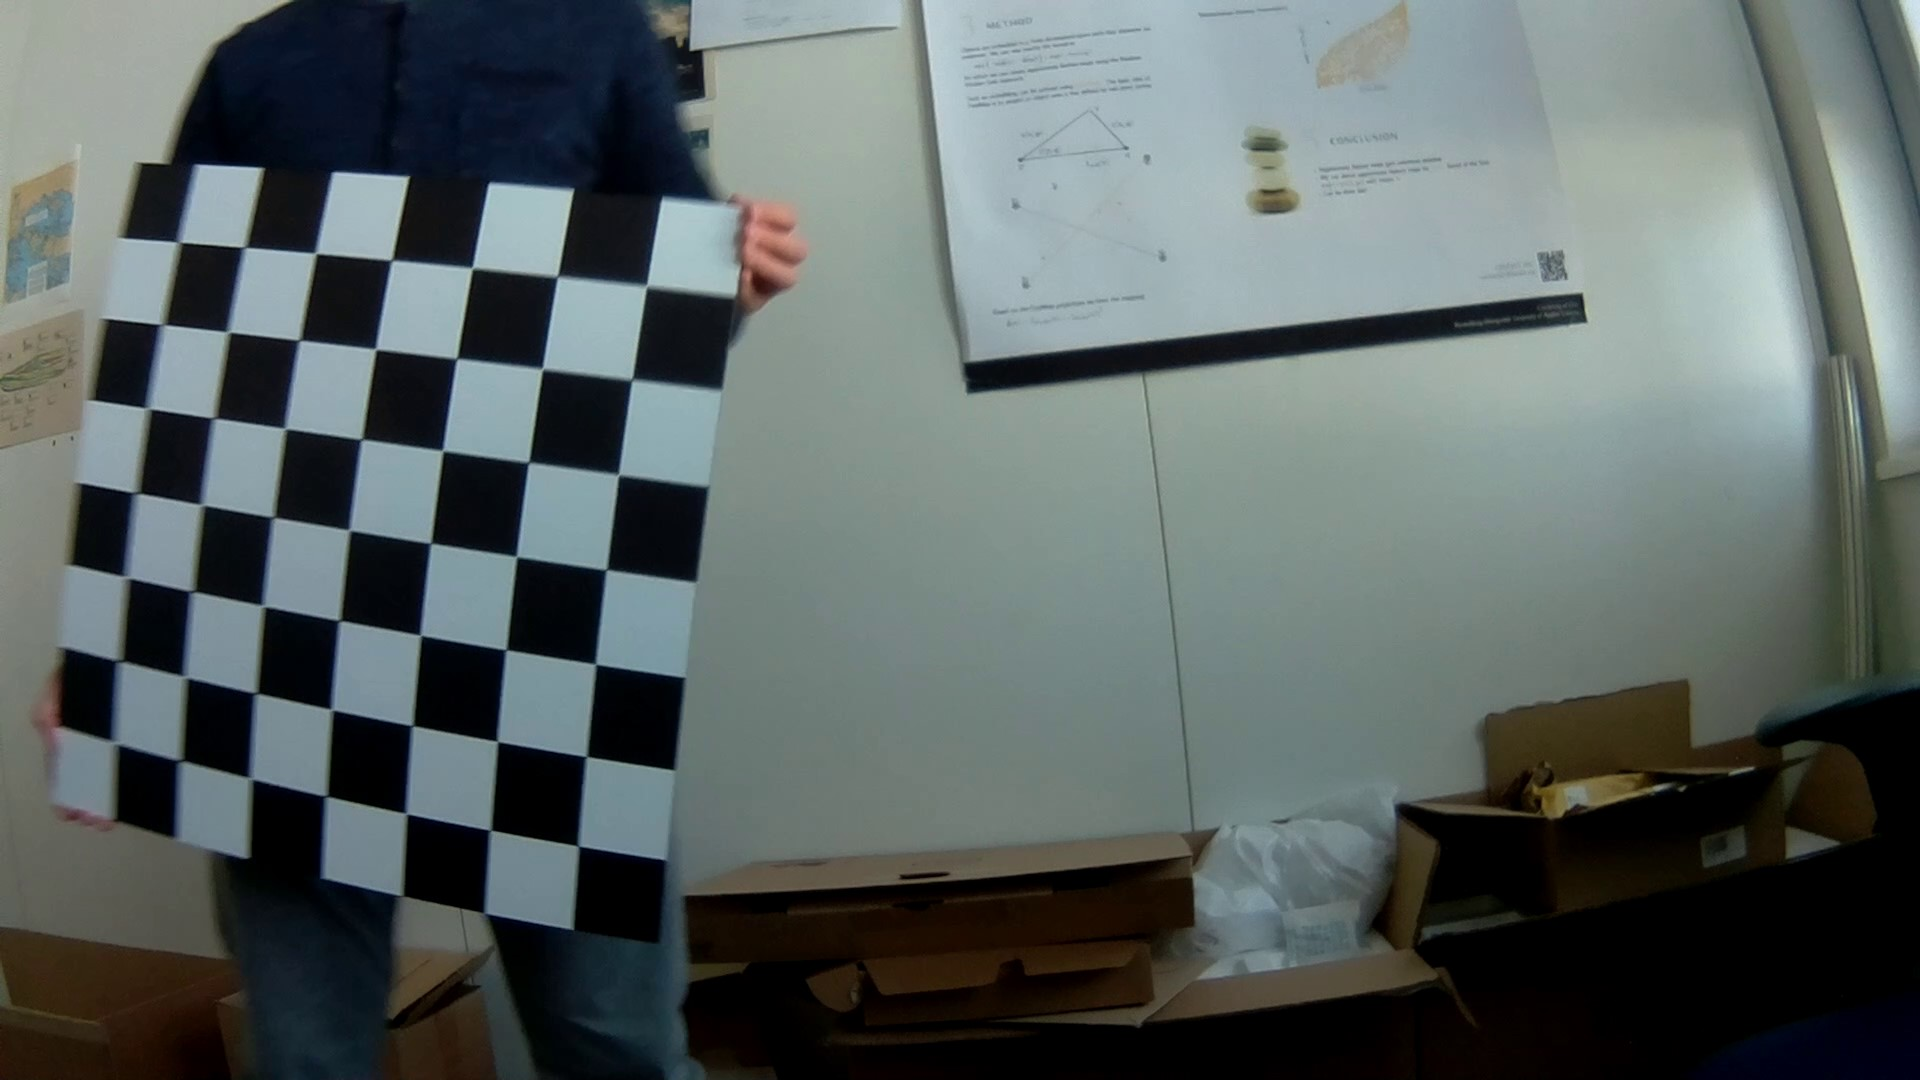
\includegraphics[width=\textwidth]{figures/img1_0.jpg}
        \caption{Distorted frame}
    \end{subfigure}
    \hfill
    \begin{subfigure}[b]{0.48\textwidth}
        \centering
        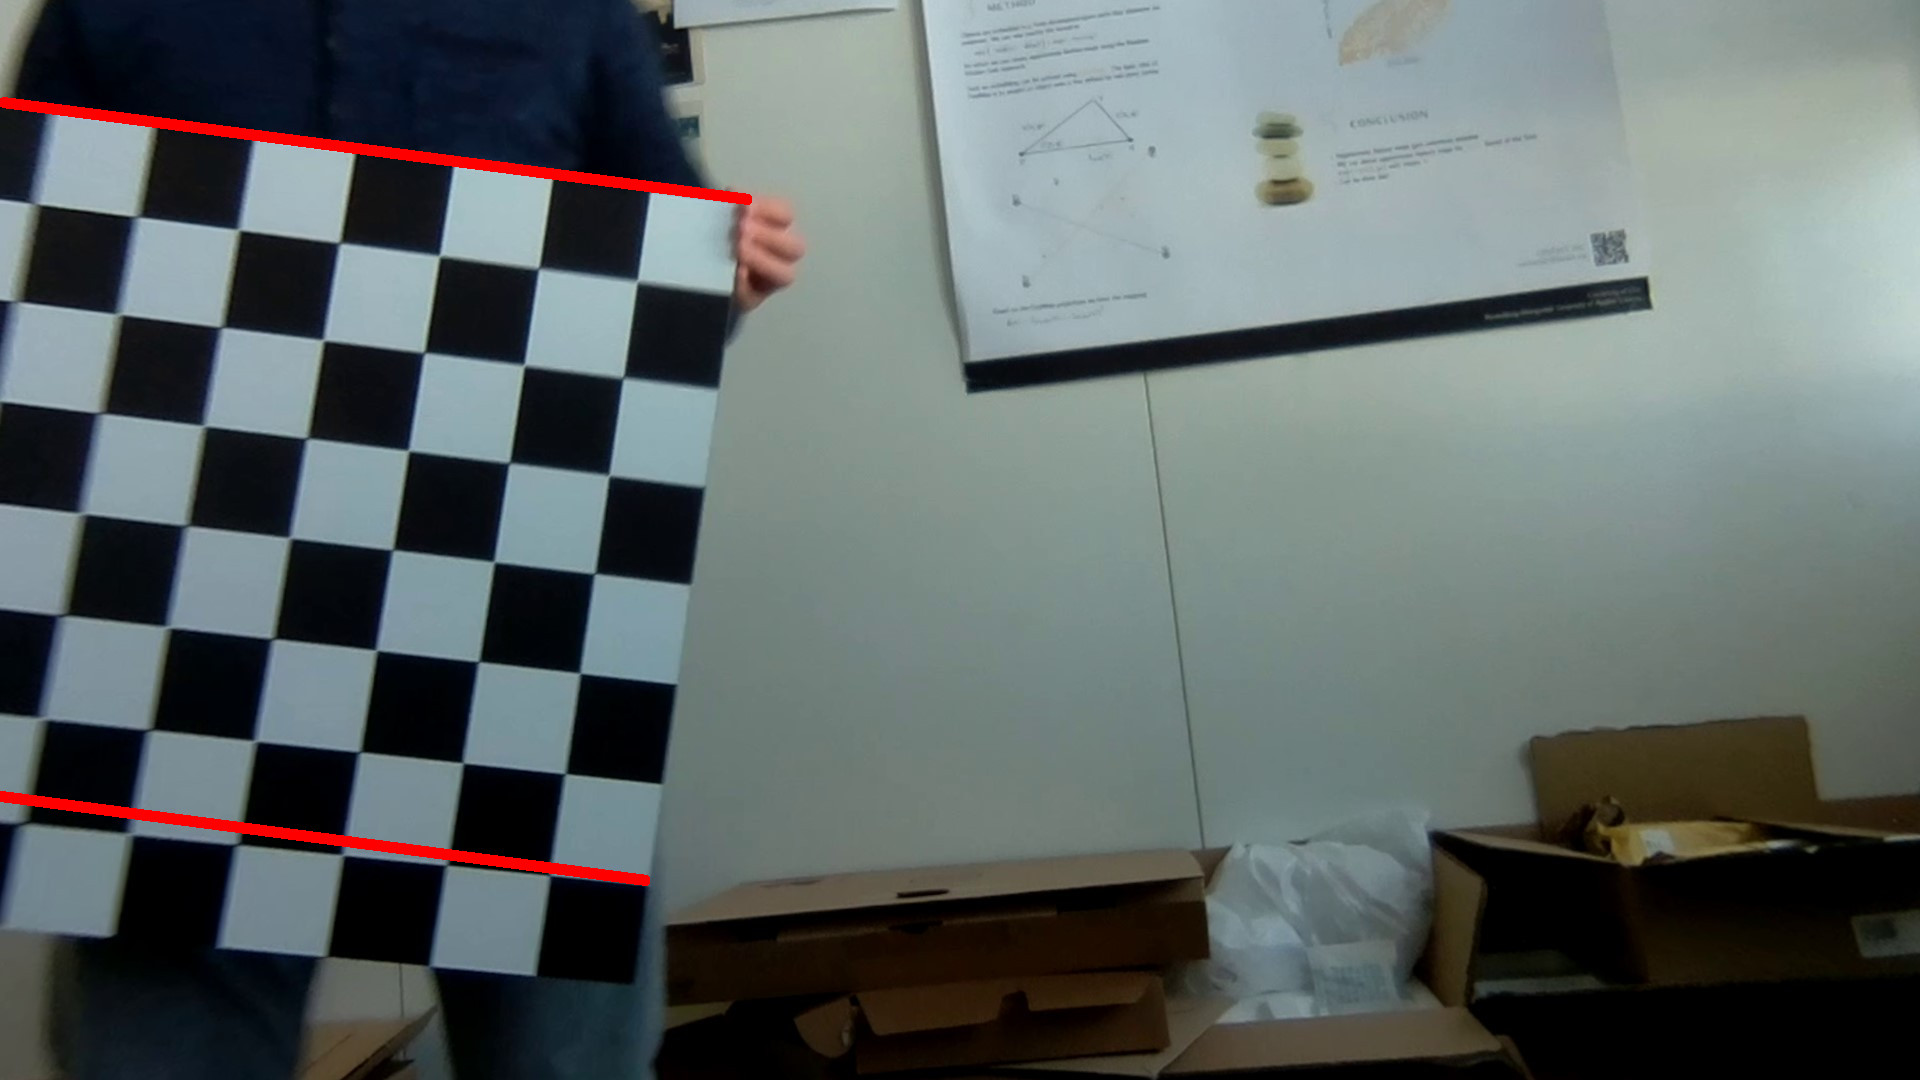
\includegraphics[width=\textwidth]{figures/img1_1.jpg}
        \caption{Undistorted frame with parallel lines}
    \end{subfigure}
    \caption{Undistortion result of video 1 frame with intrinsic matrix}
    \label{fig:dist1}
\end{figure}

The undistortion results in image pixels being lost, especially at the corners where the distortion effect is the biggest. But the chessboard lines seem to be \enquote{more parallel} than before, although not perfect - as the drawn in parallel red lines do not exactly match the chessboard pattern. The radial distortion is also reduced but not gone completely.

To reduce the amount of pixels cut away, the camera matrix can be refined using the \texttt{getOptimalNewCameraMatrix()} function of OpenCV. It accepts a parameter $0 \leq \alpha \leq 1$ that determines what should happen with the \enquote{excess} image pixels. \cite{cv_calibratecamera} A value close to 0 will discard most excess image pixels and crop into the image, while a value close to 1 will keep the excess pixels and instead fill the missing information with black pixels. A comparison between the results of different $\alpha$ values can be seen in \autoref{fig:dist2}.

\begin{figure}[h]
    \centering
    \begin{subfigure}[b]{0.3\textwidth}
        \centering
        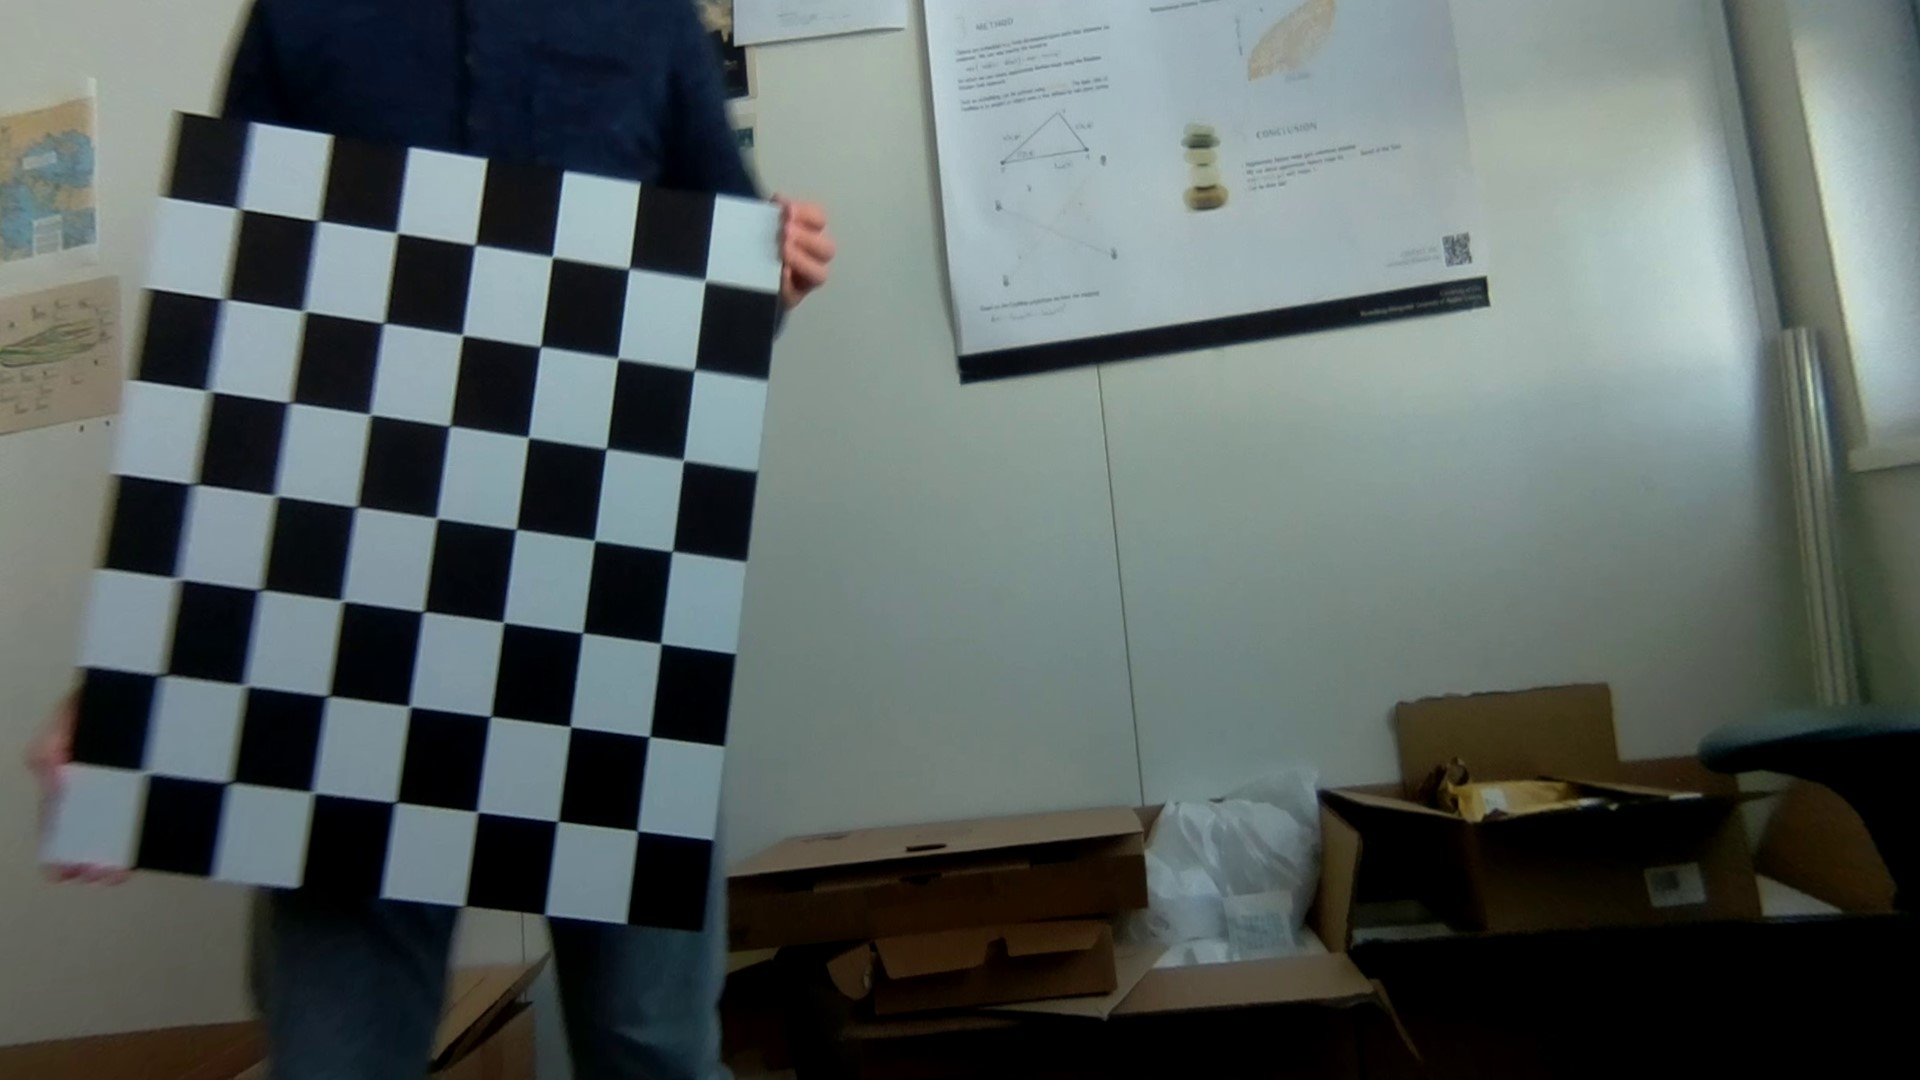
\includegraphics[width=\textwidth]{figures/img1_2.jpg}
        \caption{$\alpha = 0$}
        \label{fig:dist2a}
    \end{subfigure}
    \hfill
    \begin{subfigure}[b]{0.3\textwidth}
        \centering
        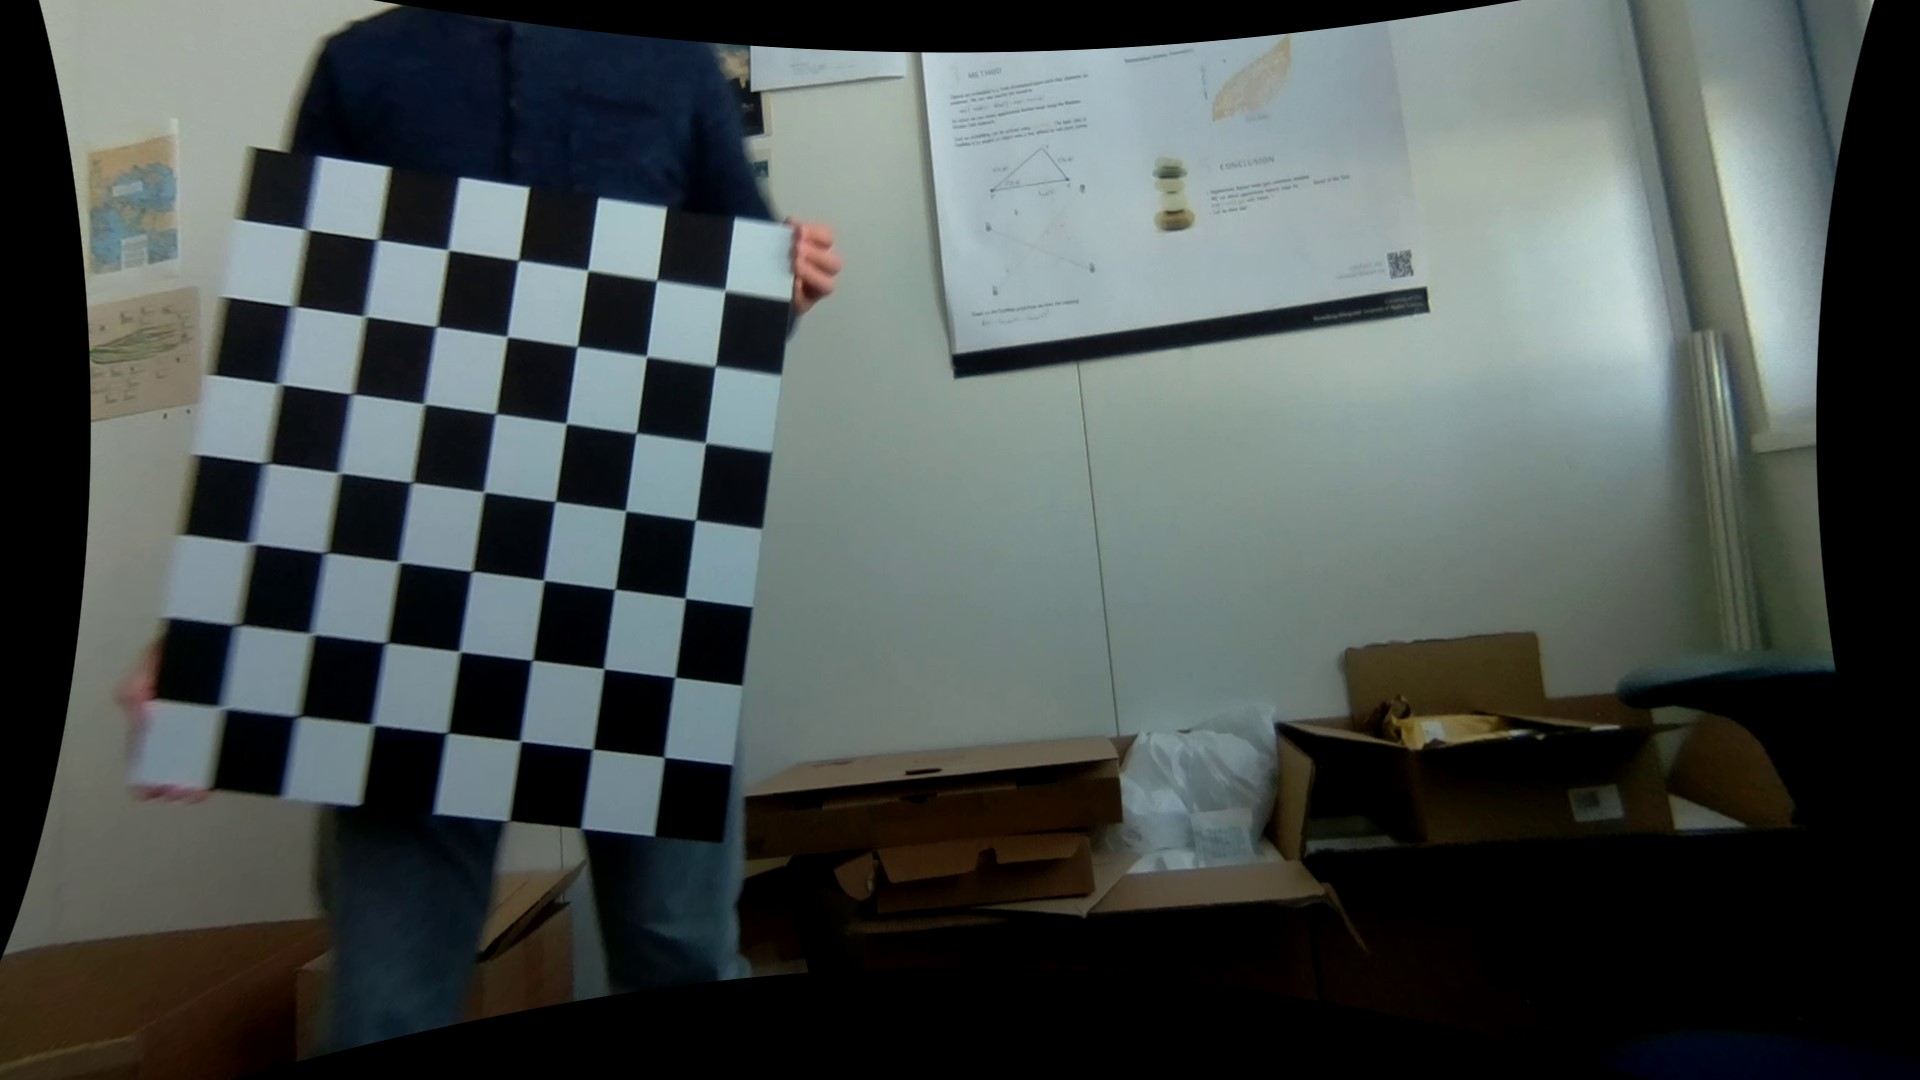
\includegraphics[width=\textwidth]{figures/img1_3.jpg}
        \caption{$\alpha = 0.5$}
    \end{subfigure}
    \hfill
    \begin{subfigure}[b]{0.3\textwidth}
        \centering
        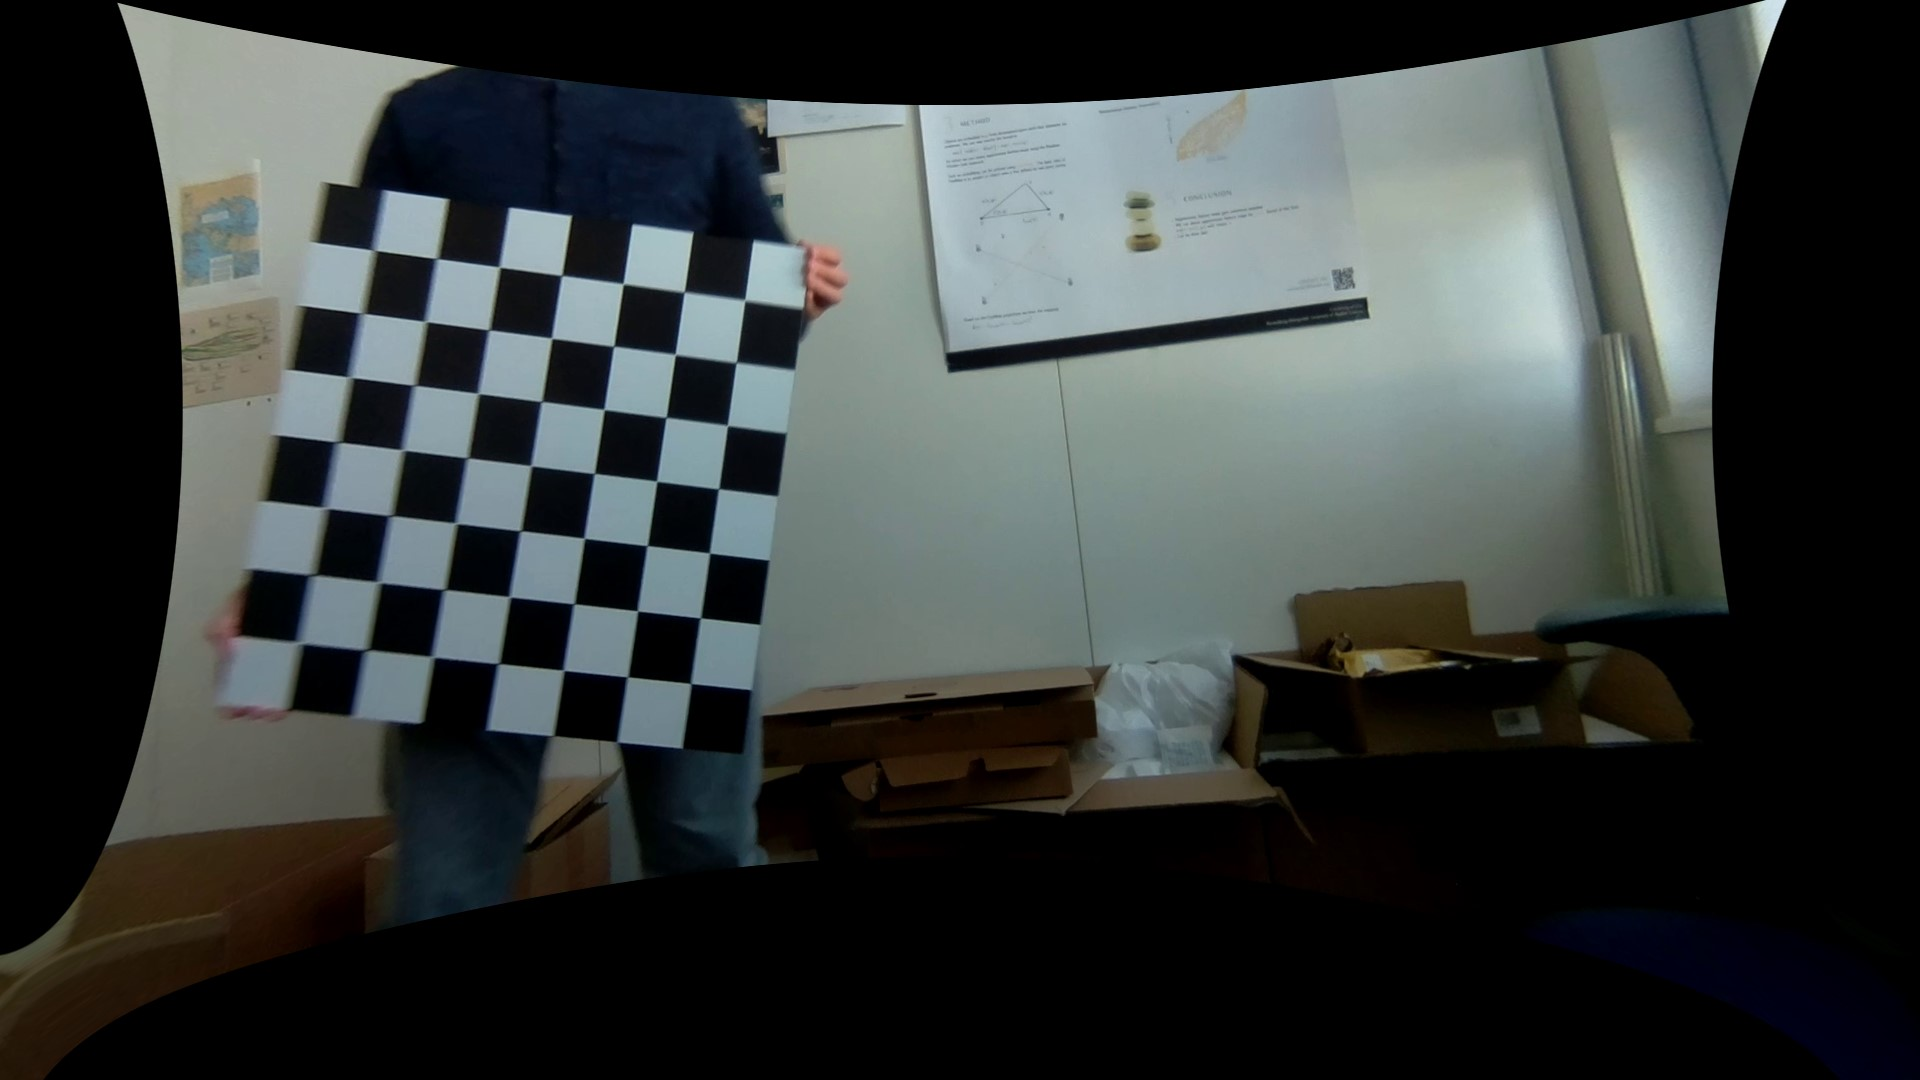
\includegraphics[width=\textwidth]{figures/img1_4.jpg}
        \caption{$\alpha = 1$}
    \end{subfigure}
    \caption{Undistortion result of video 1 frame with refined intrinsic matrix}
    \label{fig:dist2}
\end{figure}

If the black pixels should be removed now, the \texttt{getOptimalNewCameraMatrix()} function also returns a points of a rectangle which to it can be cropped to, so the resulting image contains all valid pixels for the given $\alpha$. Since $\alpha = 1$ keeps most information intact after cropping, $\alpha = 1$ will be used for all following undistortions. The end result of this cropping process can be seen in \autoref{fig:dist3}.

\begin{figure}[h]
    \centering
    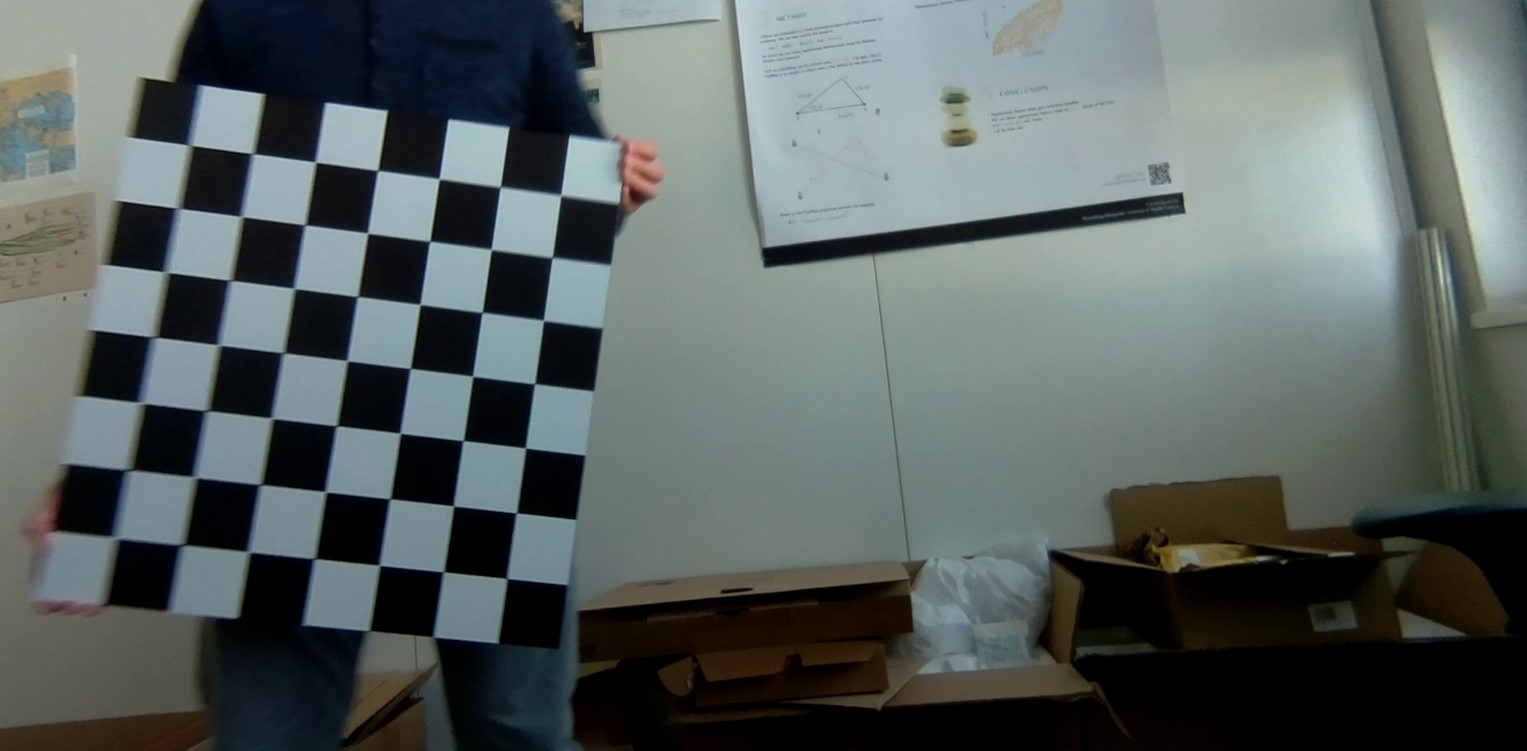
\includegraphics[width=\textwidth]{figures/img1_5.jpg}
    \caption{Cropped undistortion result of video 1 frame with refined intrinsic matrix ($\alpha = 1$)}
    \label{fig:dist3}
\end{figure}

If \autoref{fig:dist2a} and \autoref{fig:dist3} are compared, only the latter image has a correct square chessboard, while the first image is slightly streched vertically, making the chessboard rectangular and not square.

It is also noticable that in all the frames randomly selected of video 2, the chessboard is always relatively close to the camera and not farther away. This is probably due to the bad detection of the chessboard when being far away from the camera, having resulted in a higher reprojection error - making the random sample that contained these frames be filtered out.

If, regardless of that, a frame of video 2 is taken where the chessboard is far in the background (so not part of the random sample) and the undistortion with the same process as used above is applied, the image is undistorted in the same way, as expected. Since the camera used is not distorting much in the center of the image - where the chessboard is located - there is no big difference in the chessboard size and parallelism, as seen in \autoref{fig:dist4}. Nevertheless the entire environment is undistorted significantly, making the view closer to reality.

\begin{figure}[h]
    \centering
    \begin{subfigure}[b]{0.48\textwidth}
        \centering
        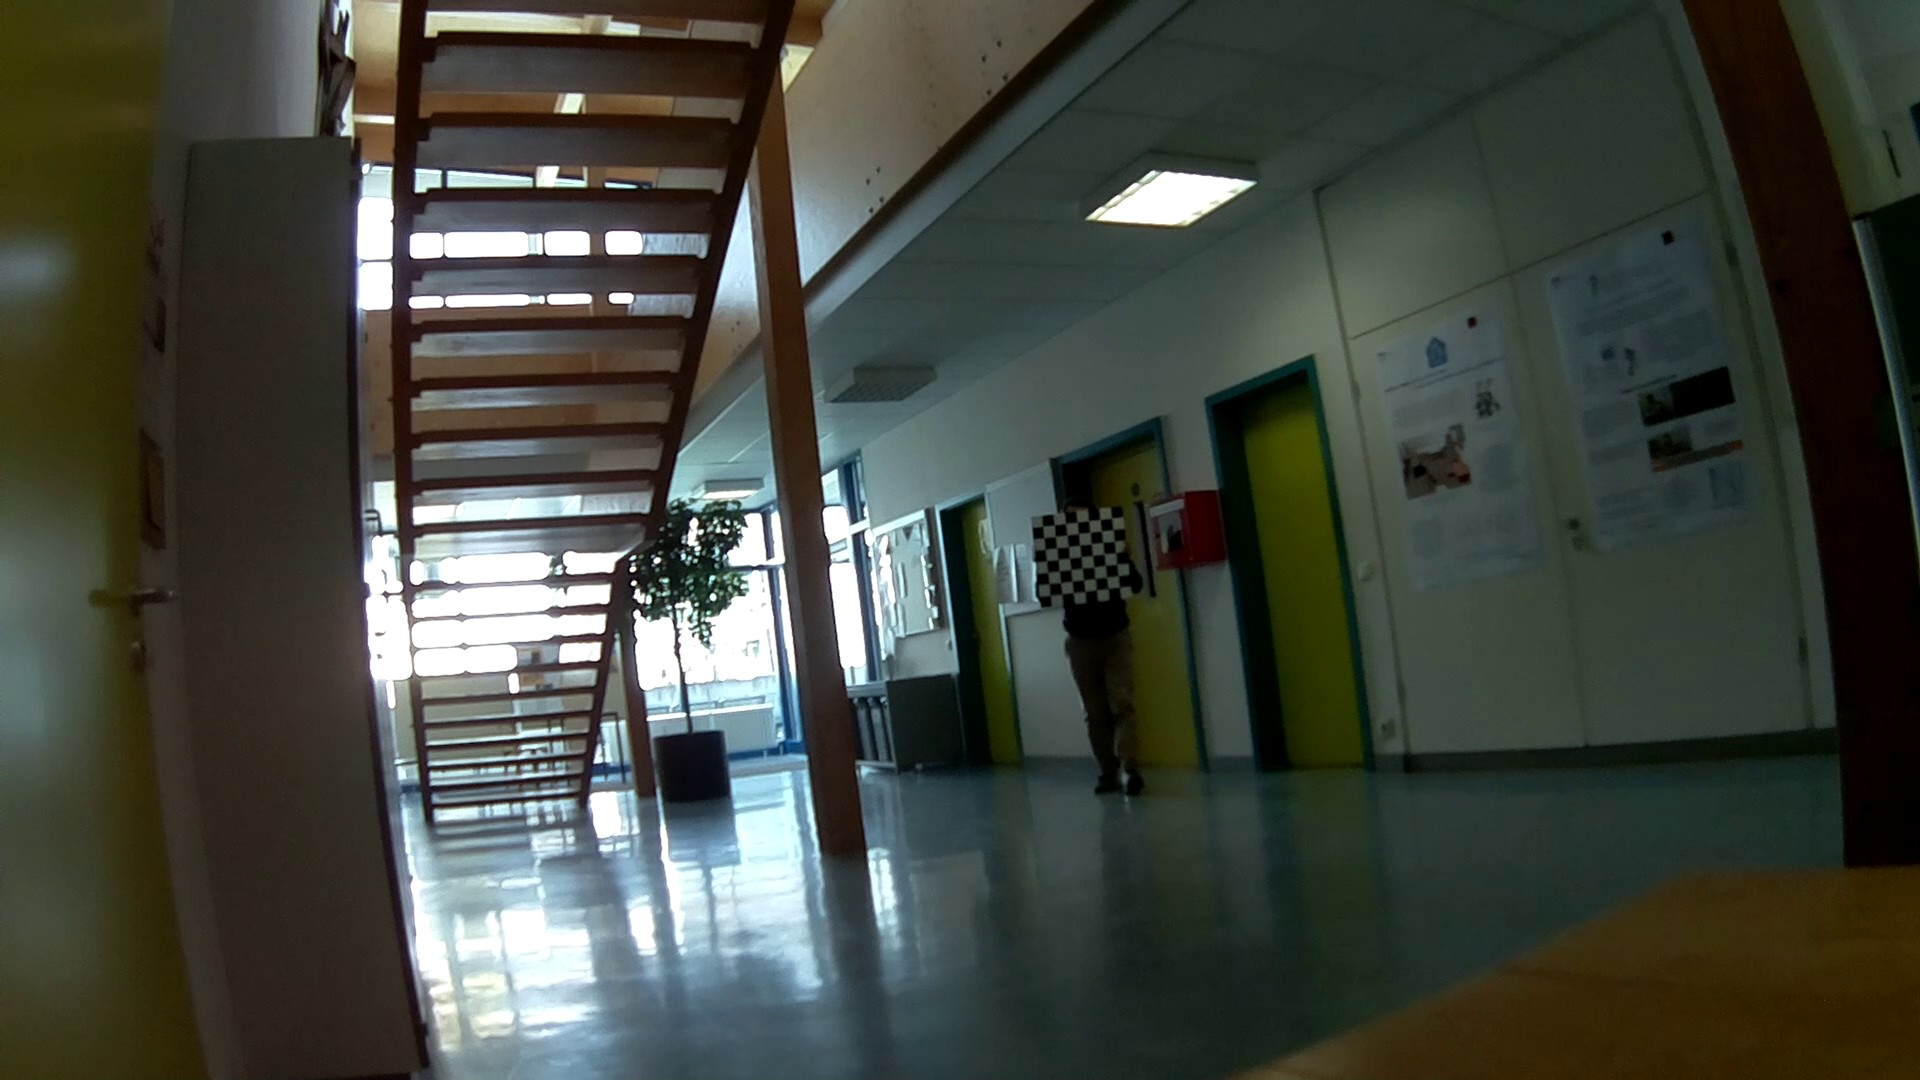
\includegraphics[width=\textwidth]{figures/img_v2_0.jpg}
        \caption{Distorted frame}
    \end{subfigure}
    \hfill
    \begin{subfigure}[b]{0.48\textwidth}
        \centering
        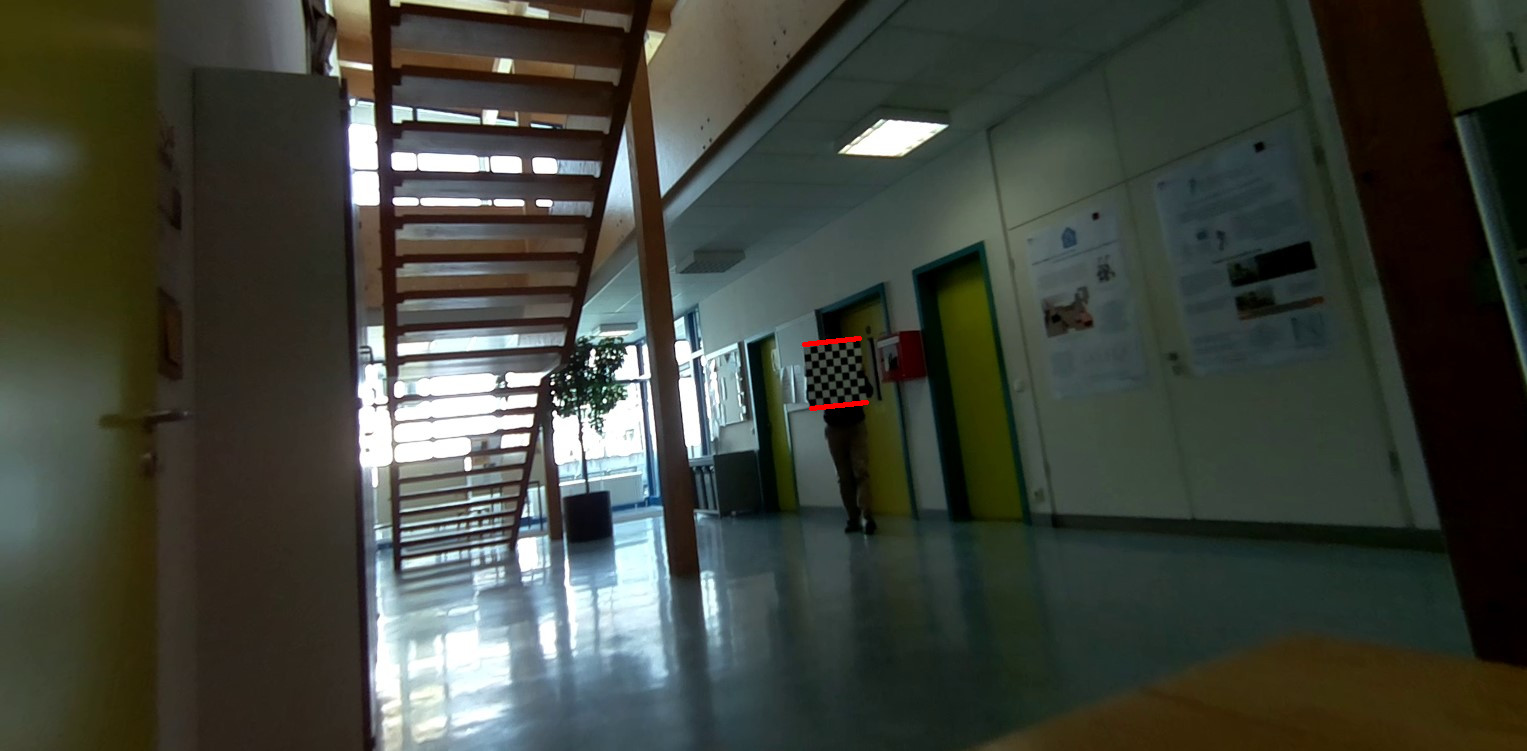
\includegraphics[width=\textwidth]{figures/img_v2_5.jpg}
        \caption{Undistorted frame with parallel lines}
    \end{subfigure}
    \caption{Undistortion result of video 2 frame (ID 450) with intrinsic matrix}
    \label{fig:dist4}
\end{figure}

\subsection{Additional undistorted images}

\begin{figure}[h]
    \centering
    \begin{subfigure}[b]{0.48\textwidth}
        \centering
        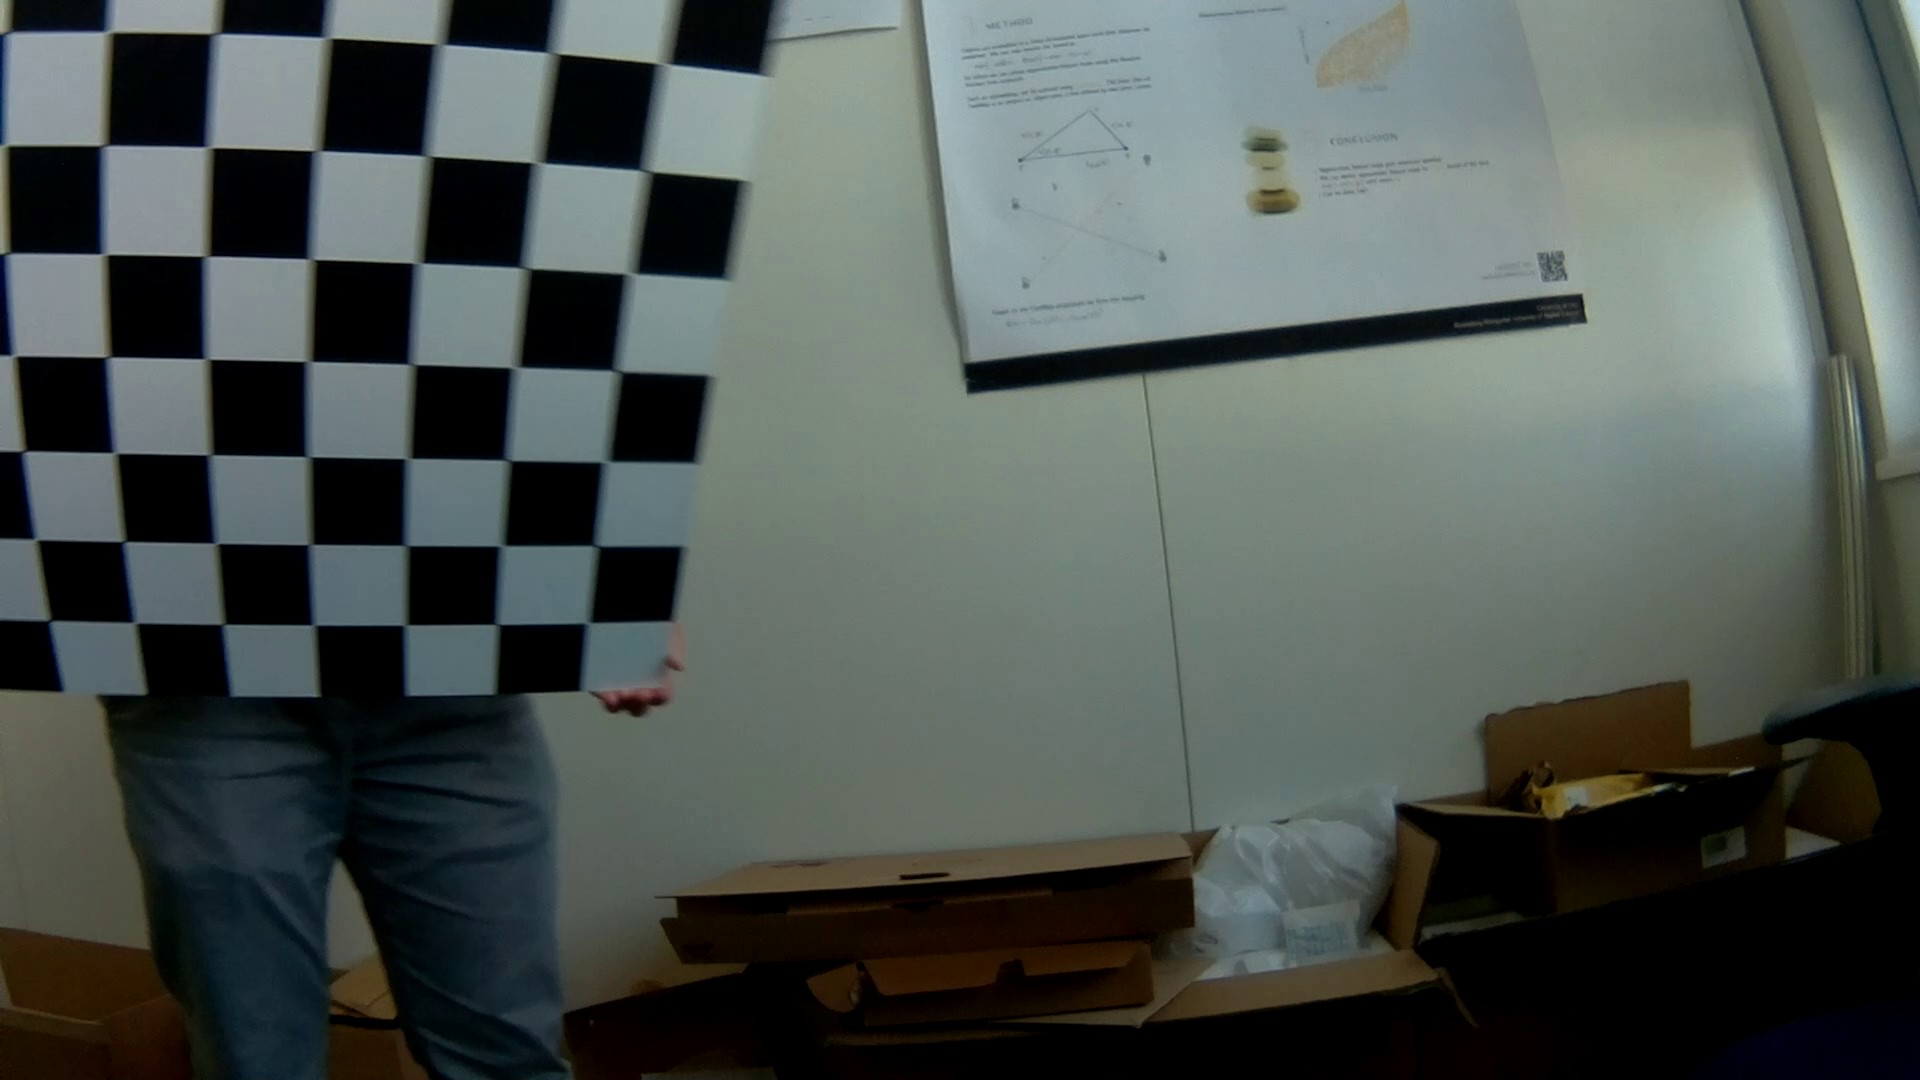
\includegraphics[width=\textwidth]{figures/addl/img4_0.jpg}
        \caption{Distorted frame}
    \end{subfigure}
    \hfill
    \begin{subfigure}[b]{0.48\textwidth}
        \centering
        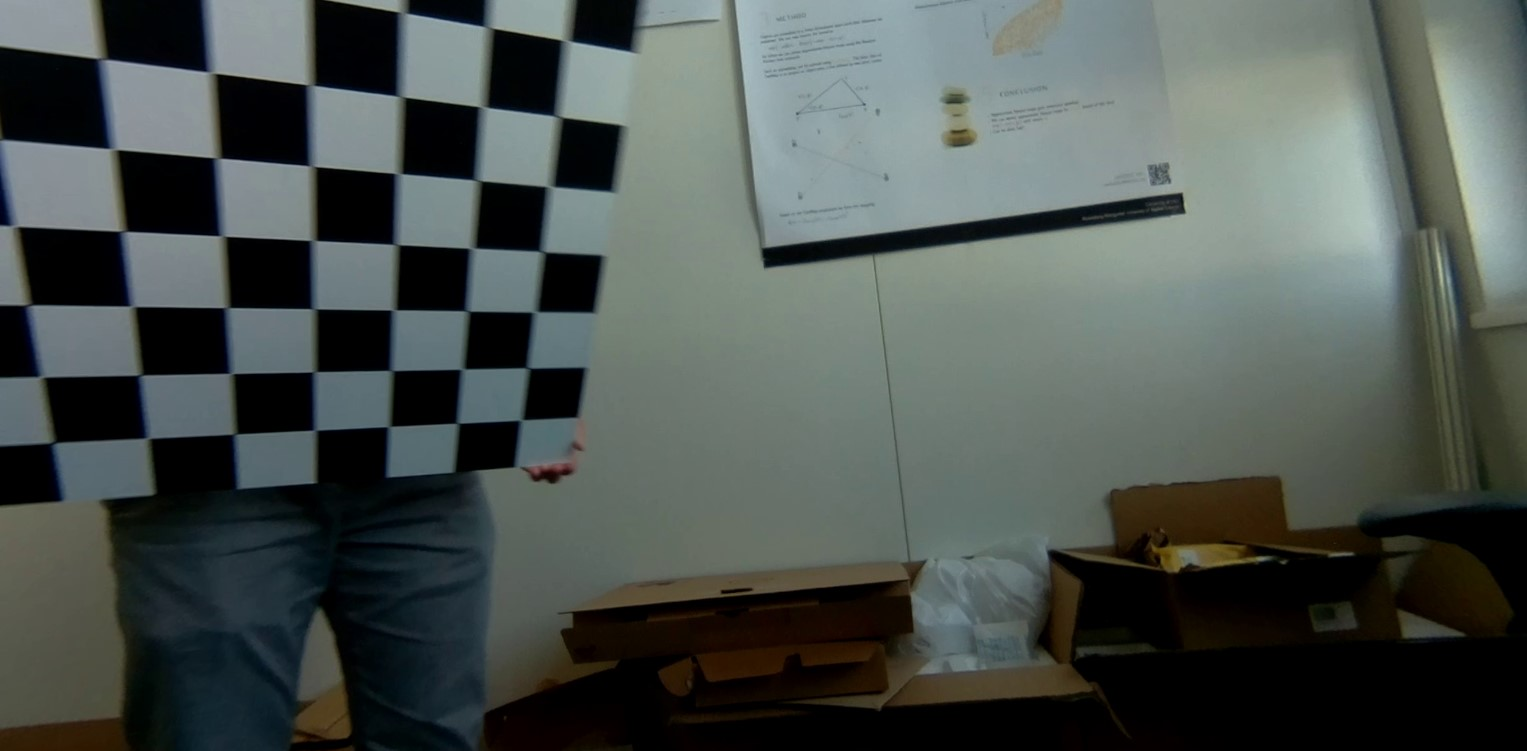
\includegraphics[width=\textwidth]{figures/addl/img4_5.jpg}
        \caption{Undistorted frame}
    \end{subfigure}
    \caption{Undistortion result of video 1 frame (2)}
    \label{fig:dist_1a2}
\end{figure}

\begin{figure}[h]
    \centering
    \begin{subfigure}[b]{0.48\textwidth}
        \centering
        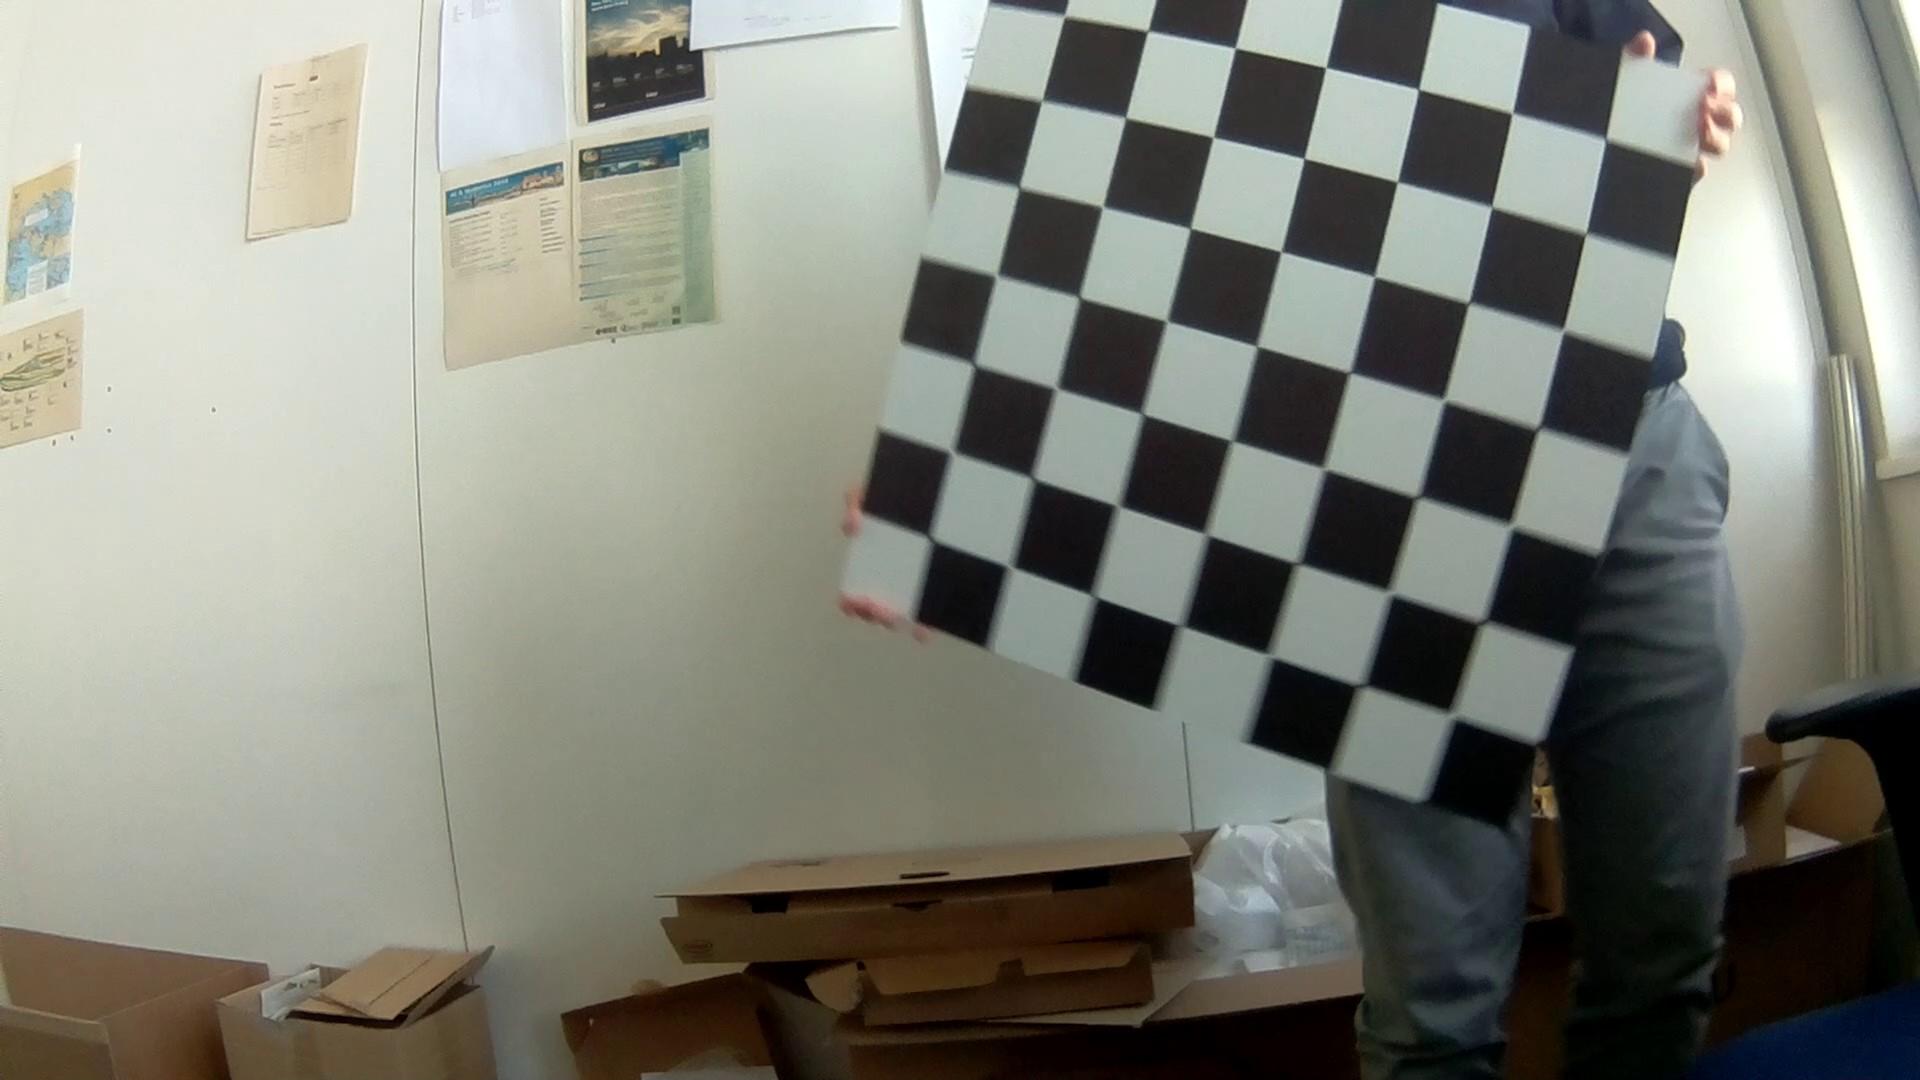
\includegraphics[width=\textwidth]{figures/addl/img5_0.jpg}
        \caption{Distorted frame}
    \end{subfigure}
    \hfill
    \begin{subfigure}[b]{0.48\textwidth}
        \centering
        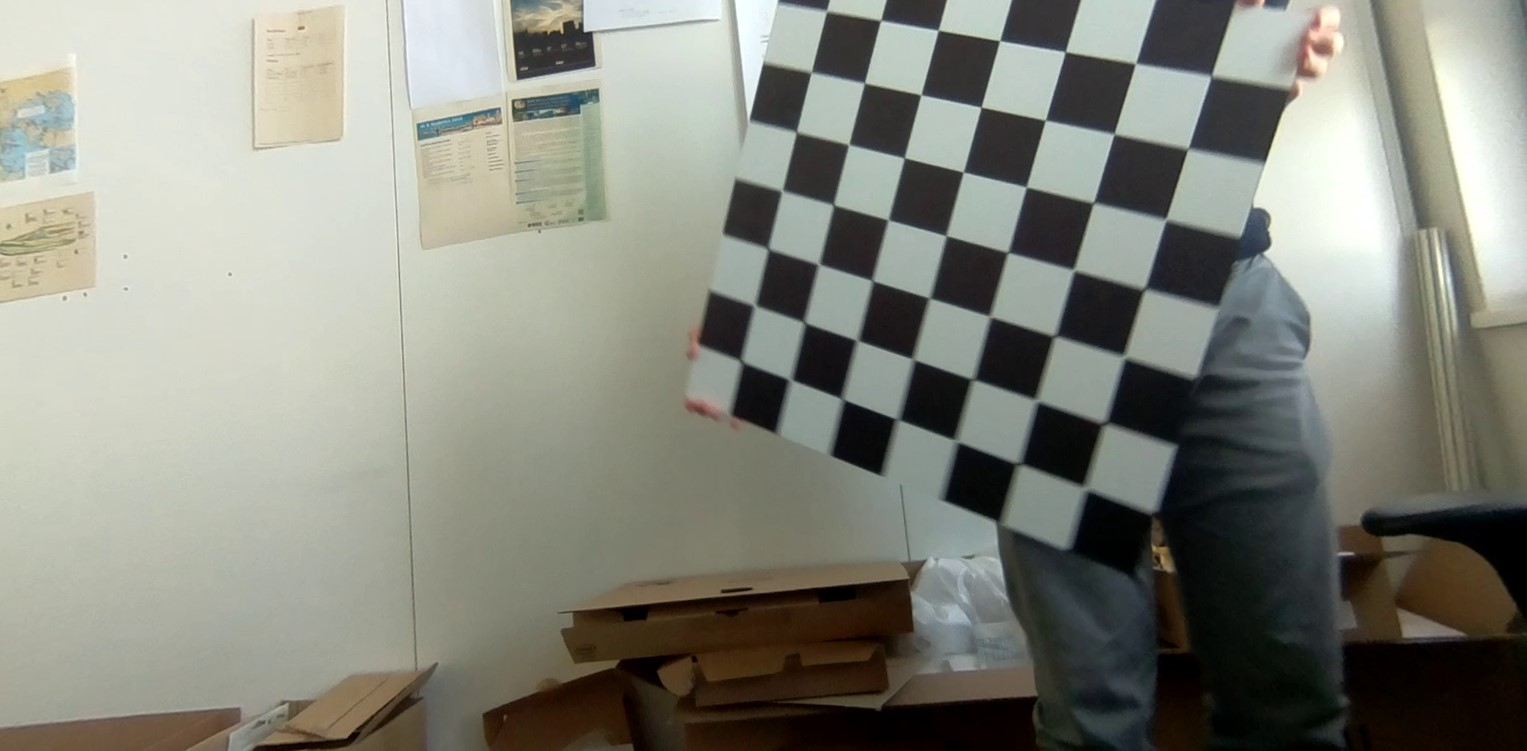
\includegraphics[width=\textwidth]{figures/addl/img5_5.jpg}
        \caption{Undistorted frame}
    \end{subfigure}
    \caption{Undistortion result of video 1 frame (3)}
    \label{fig:dist_1a3}
\end{figure}

\begin{figure}[h]
    \centering
    \begin{subfigure}[b]{0.48\textwidth}
        \centering
        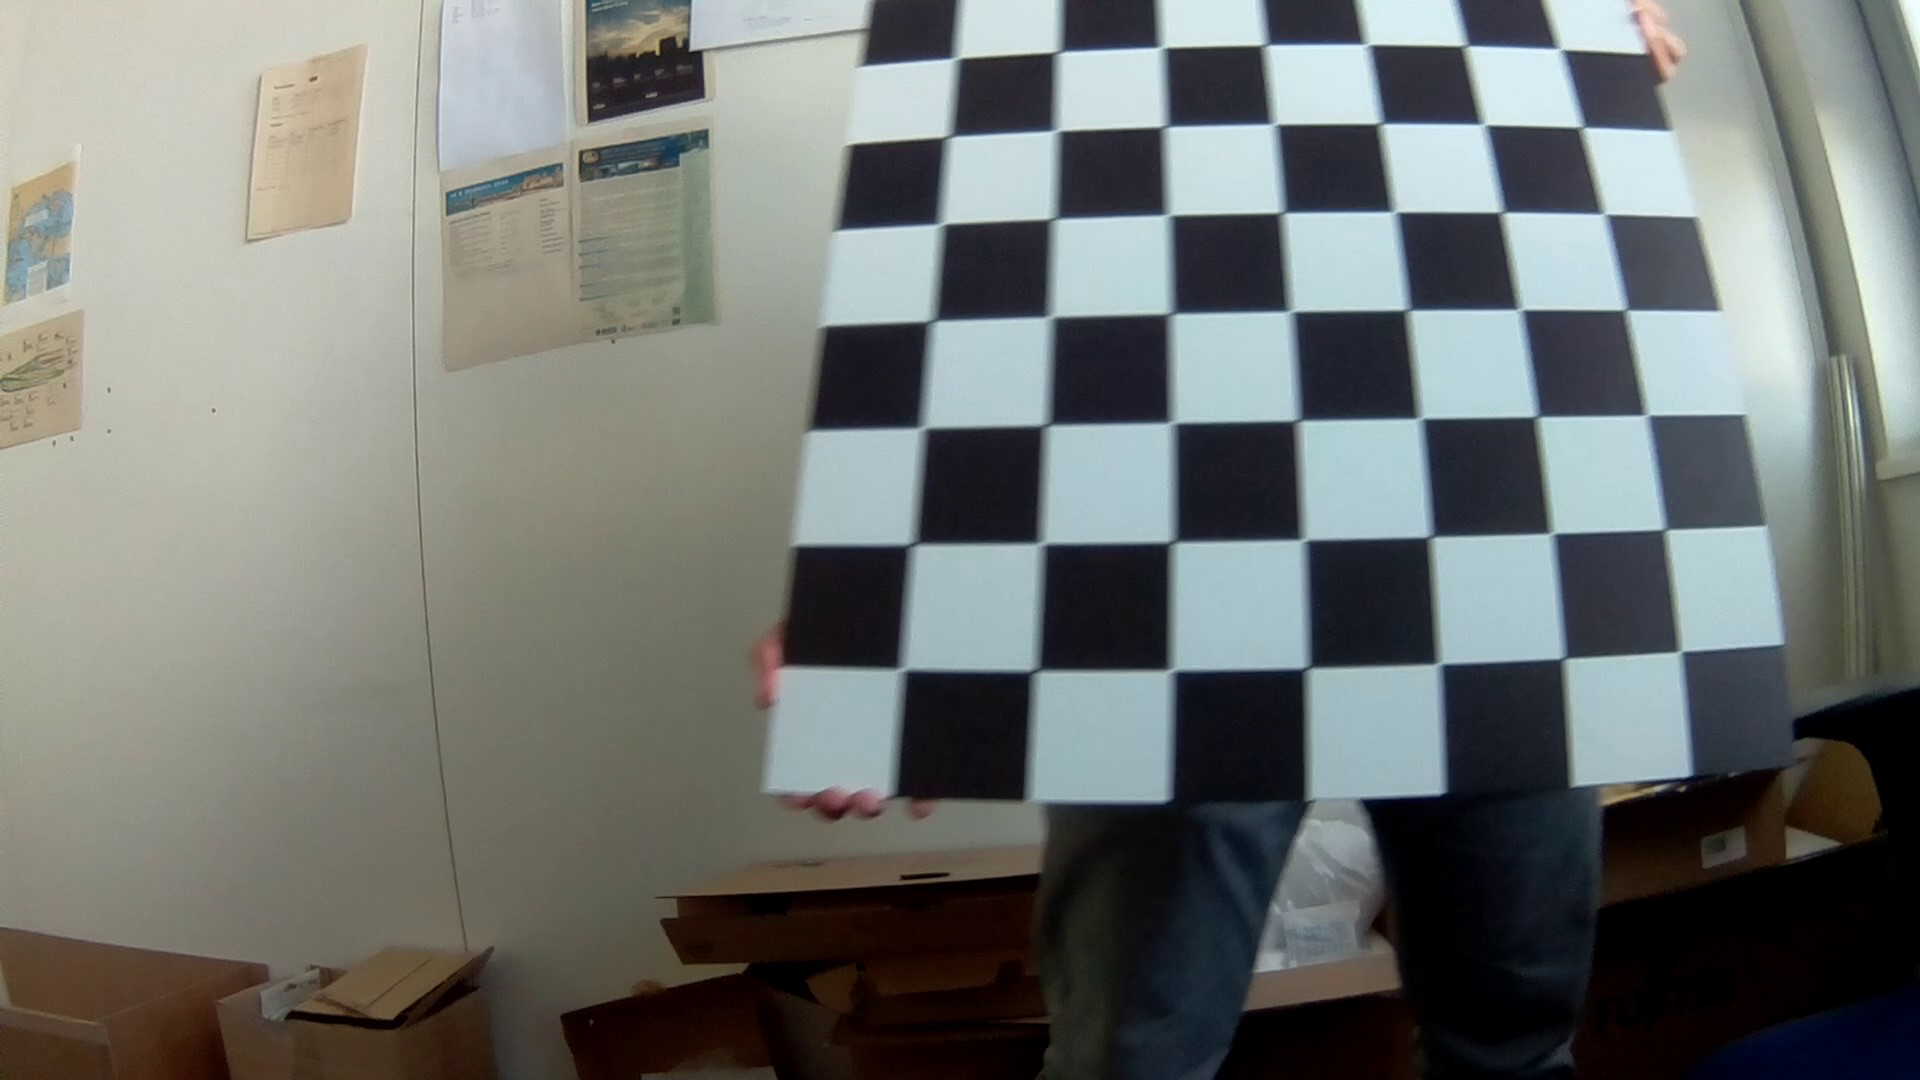
\includegraphics[width=\textwidth]{figures/addl/img8_0.jpg}
        \caption{Distorted frame}
    \end{subfigure}
    \hfill
    \begin{subfigure}[b]{0.48\textwidth}
        \centering
        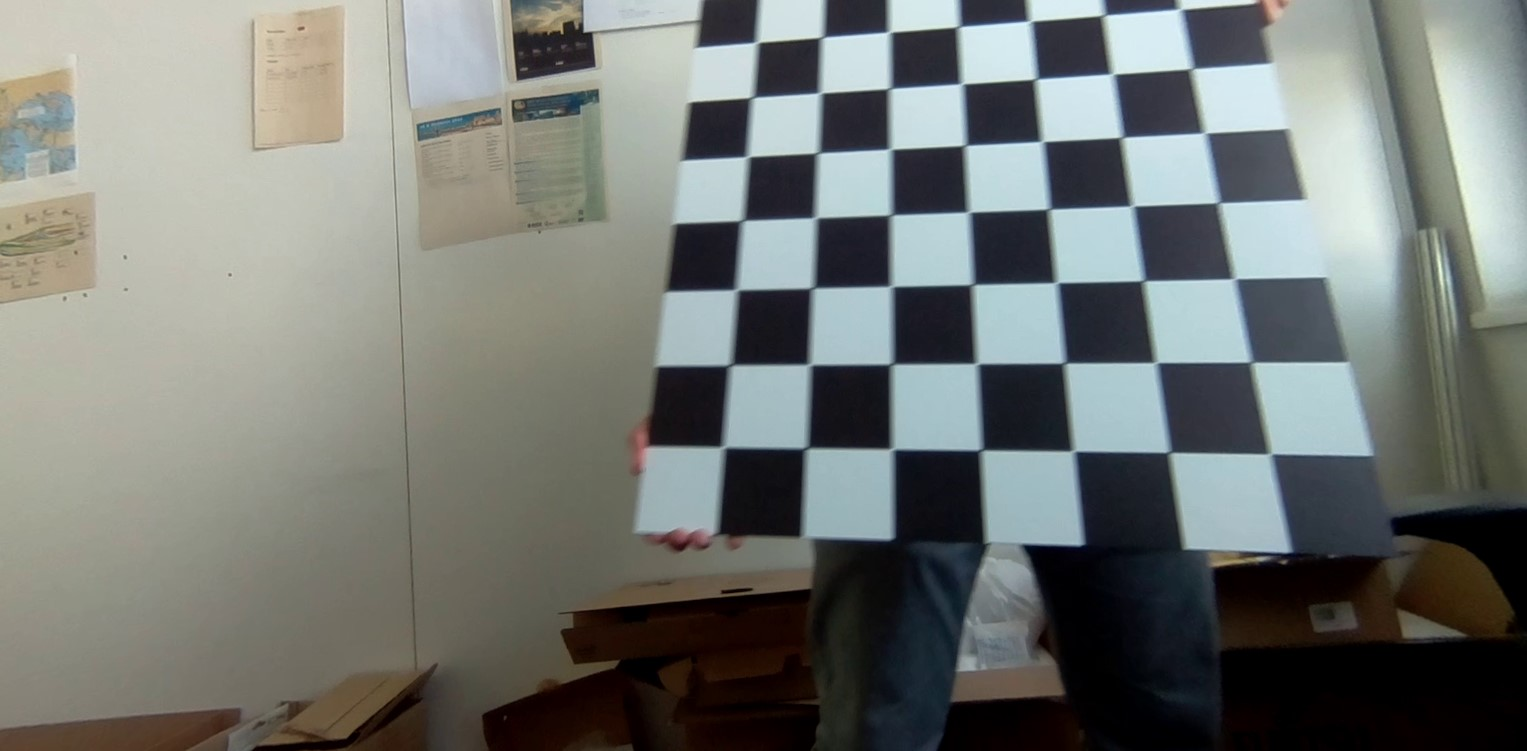
\includegraphics[width=\textwidth]{figures/addl/img8_5.jpg}
        \caption{Undistorted frame}
    \end{subfigure}
    \caption{Undistortion result of video 1 frame (4)}
    \label{fig:dist_1a4}
\end{figure}

\begin{figure}[h]
    \centering
    \begin{subfigure}[b]{0.48\textwidth}
        \centering
        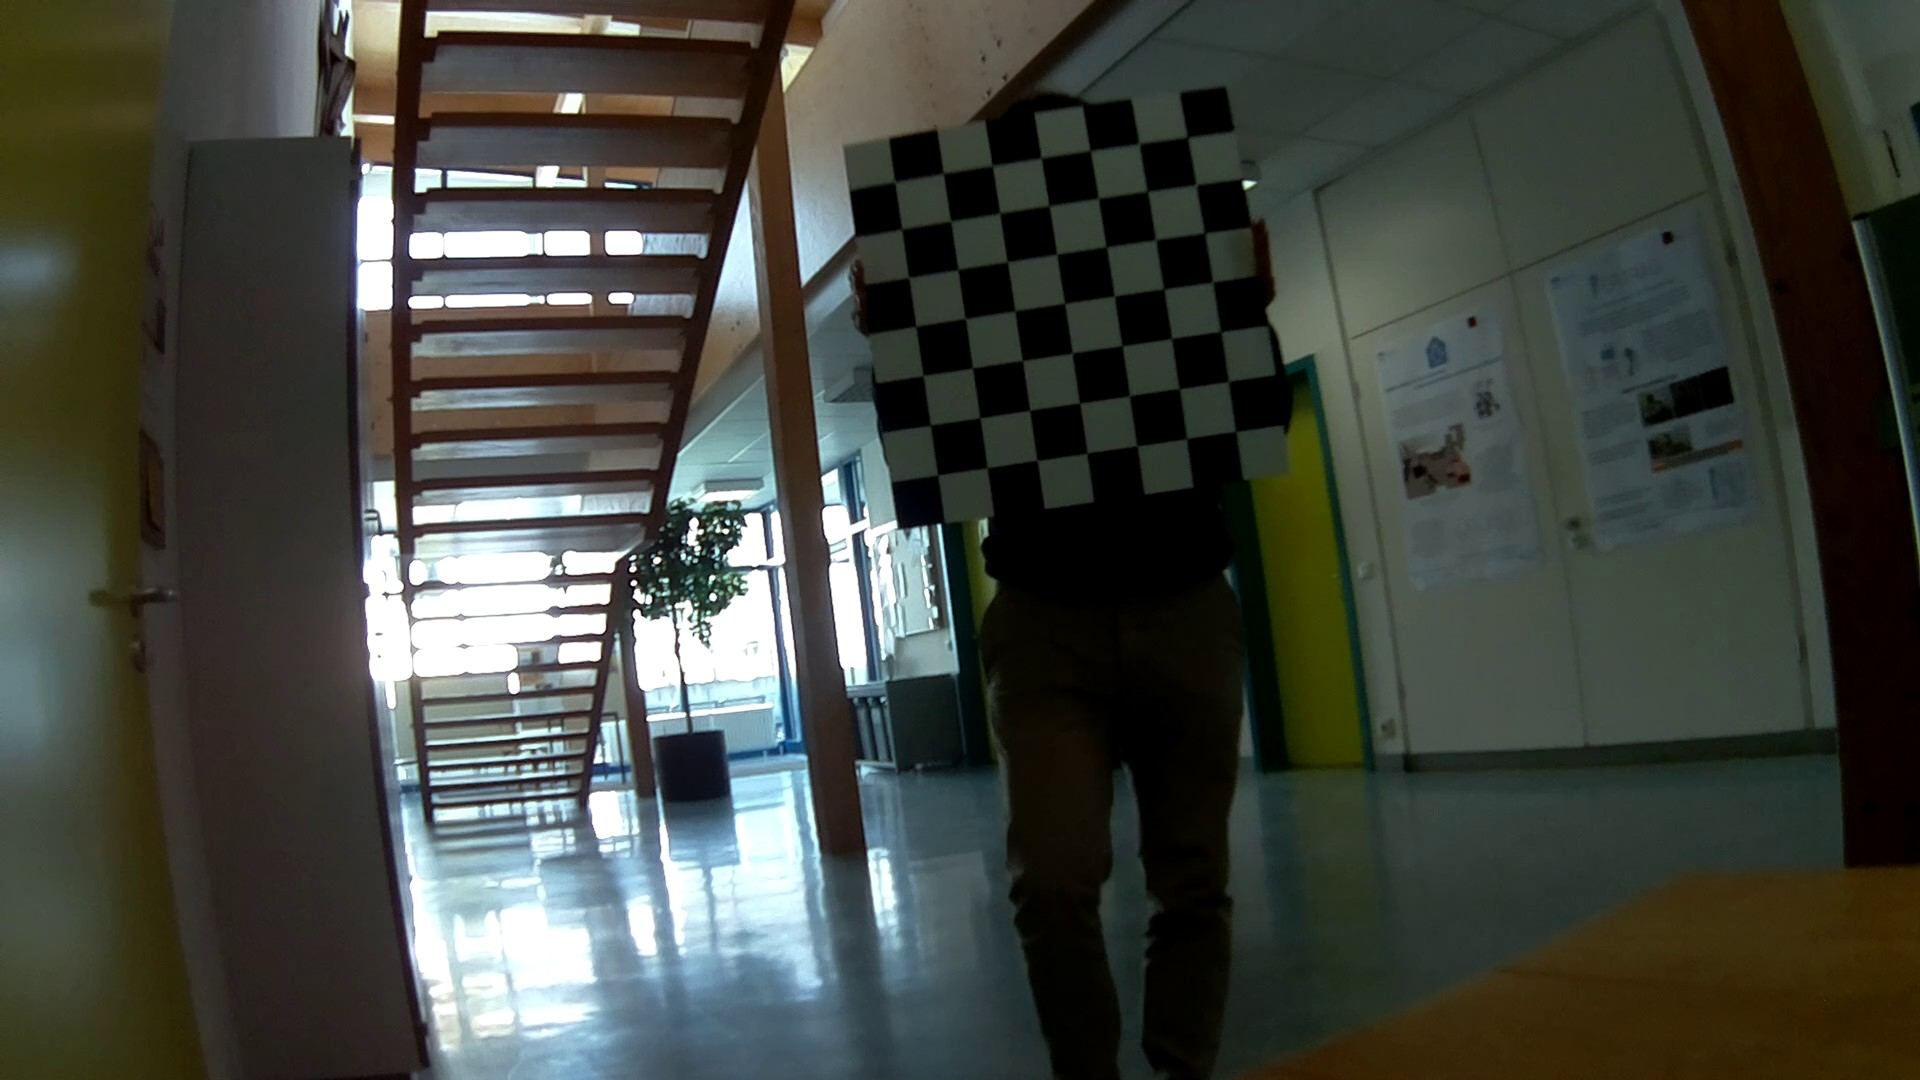
\includegraphics[width=\textwidth]{figures/addl/img10_0.jpg}
        \caption{Distorted frame}
    \end{subfigure}
    \hfill
    \begin{subfigure}[b]{0.48\textwidth}
        \centering
        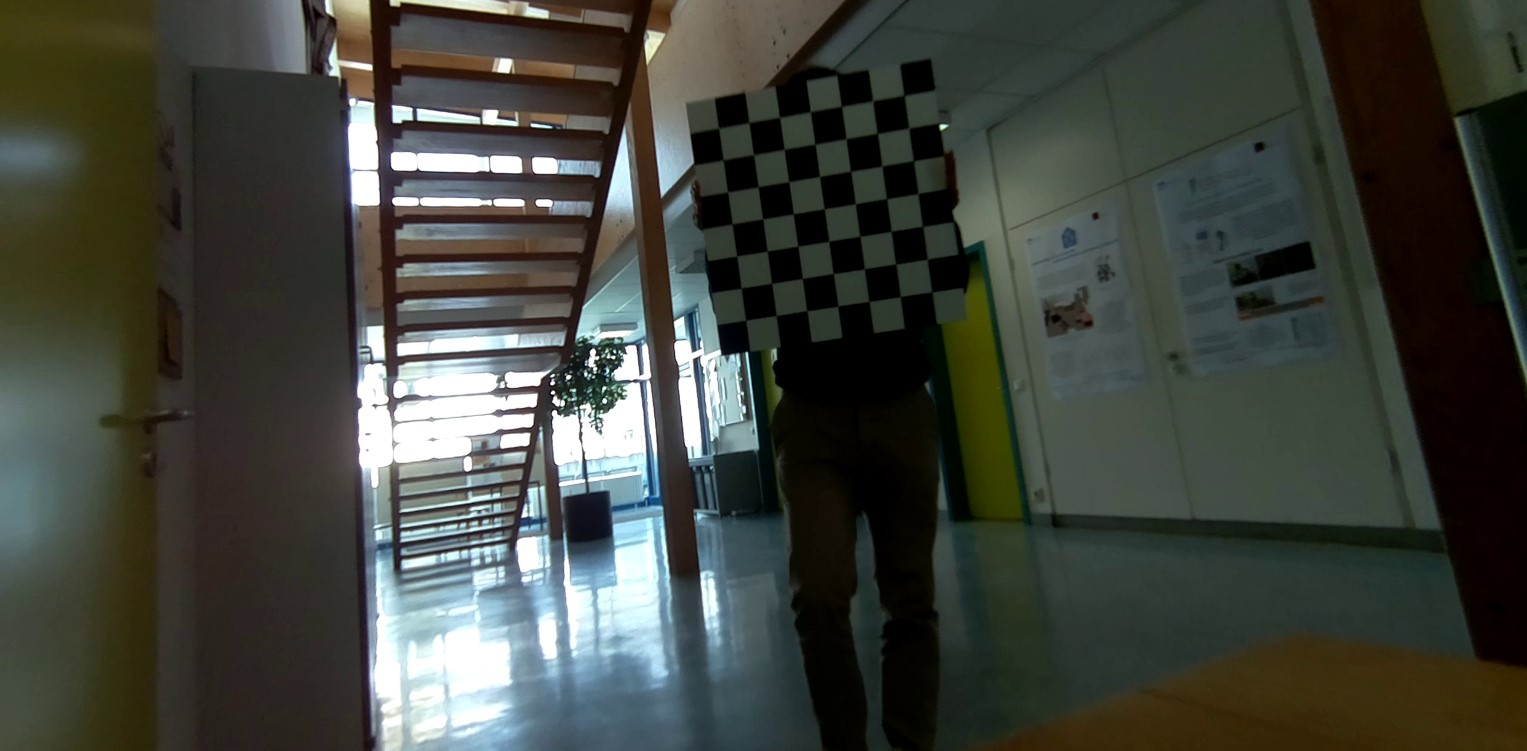
\includegraphics[width=\textwidth]{figures/addl/img10_5.jpg}
        \caption{Undistorted frame}
    \end{subfigure}
    \caption{Undistortion result of video 2 frame (2)}
    \label{fig:dist_2a2}
\end{figure}

\begin{figure}[h]
    \centering
    \begin{subfigure}[b]{0.48\textwidth}
        \centering
        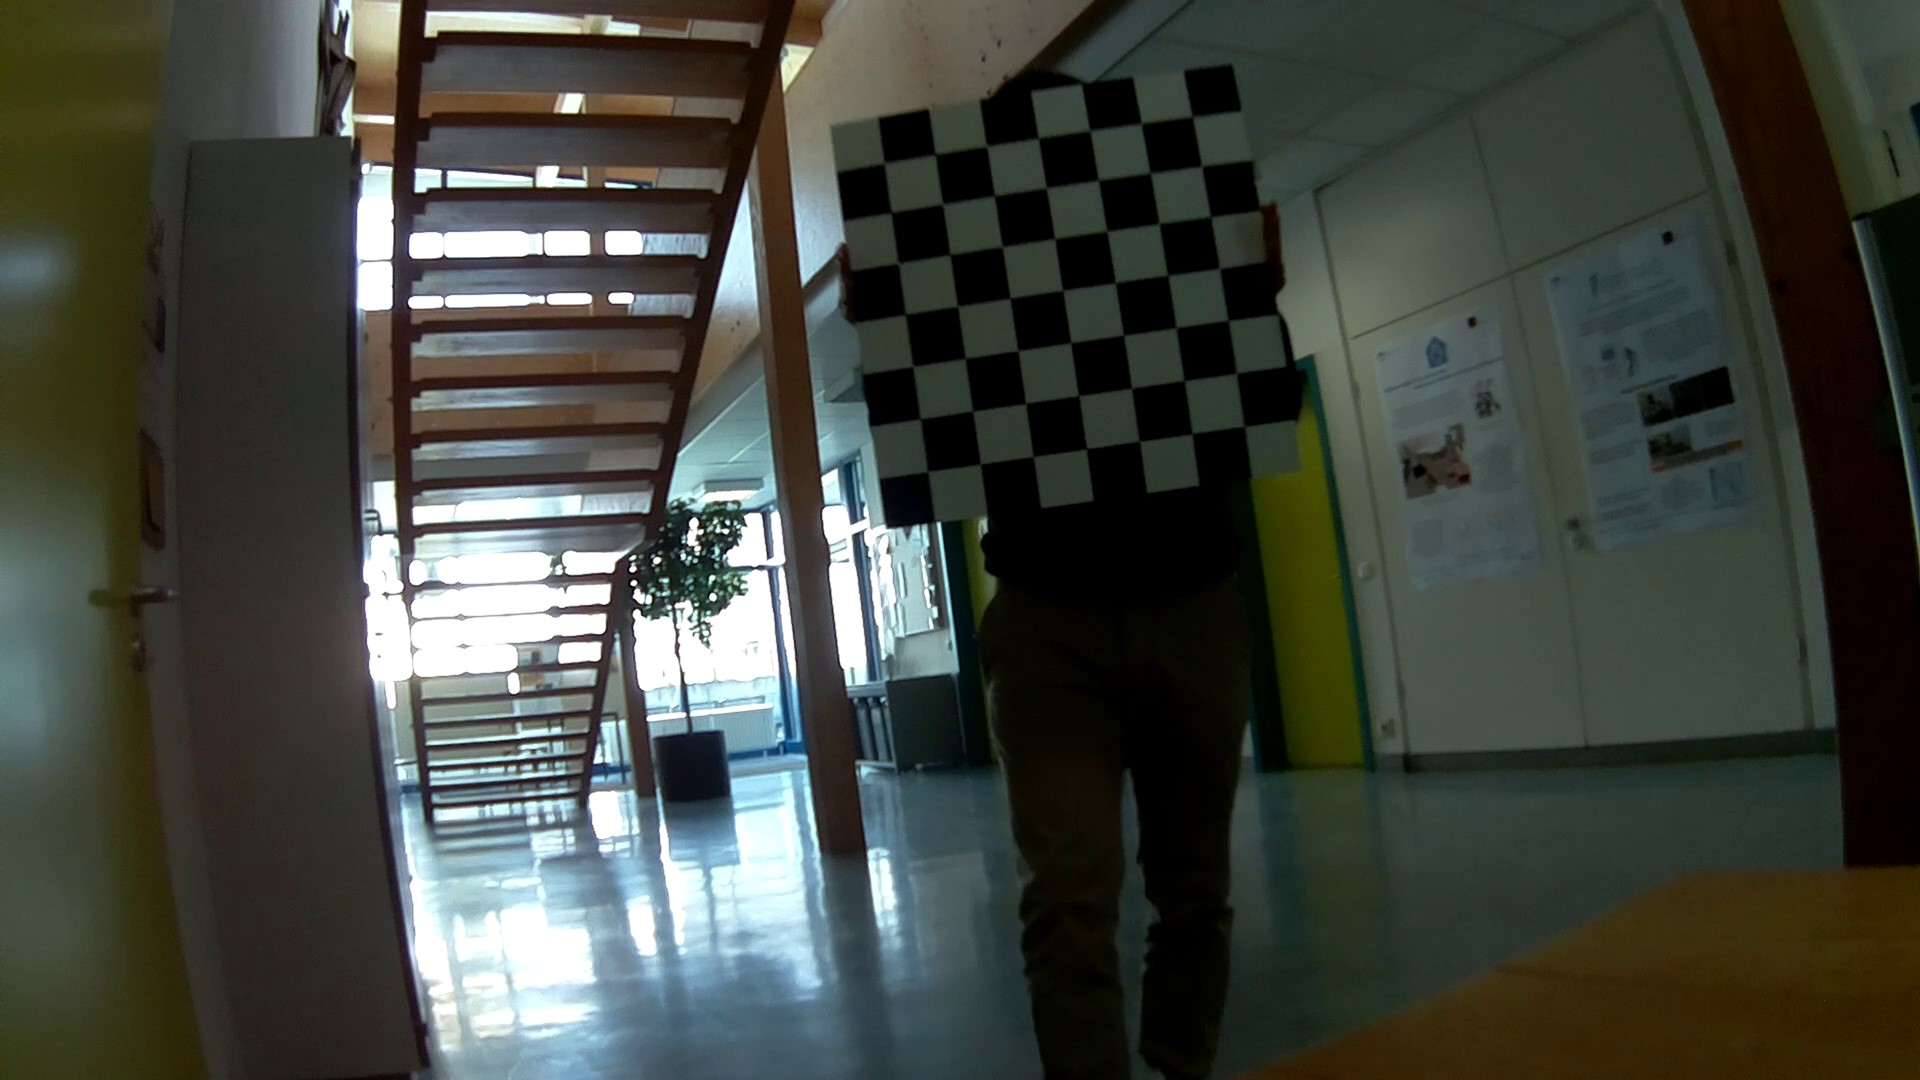
\includegraphics[width=\textwidth]{figures/addl/img13_0.jpg}
        \caption{Distorted frame}
    \end{subfigure}
    \hfill
    \begin{subfigure}[b]{0.48\textwidth}
        \centering
        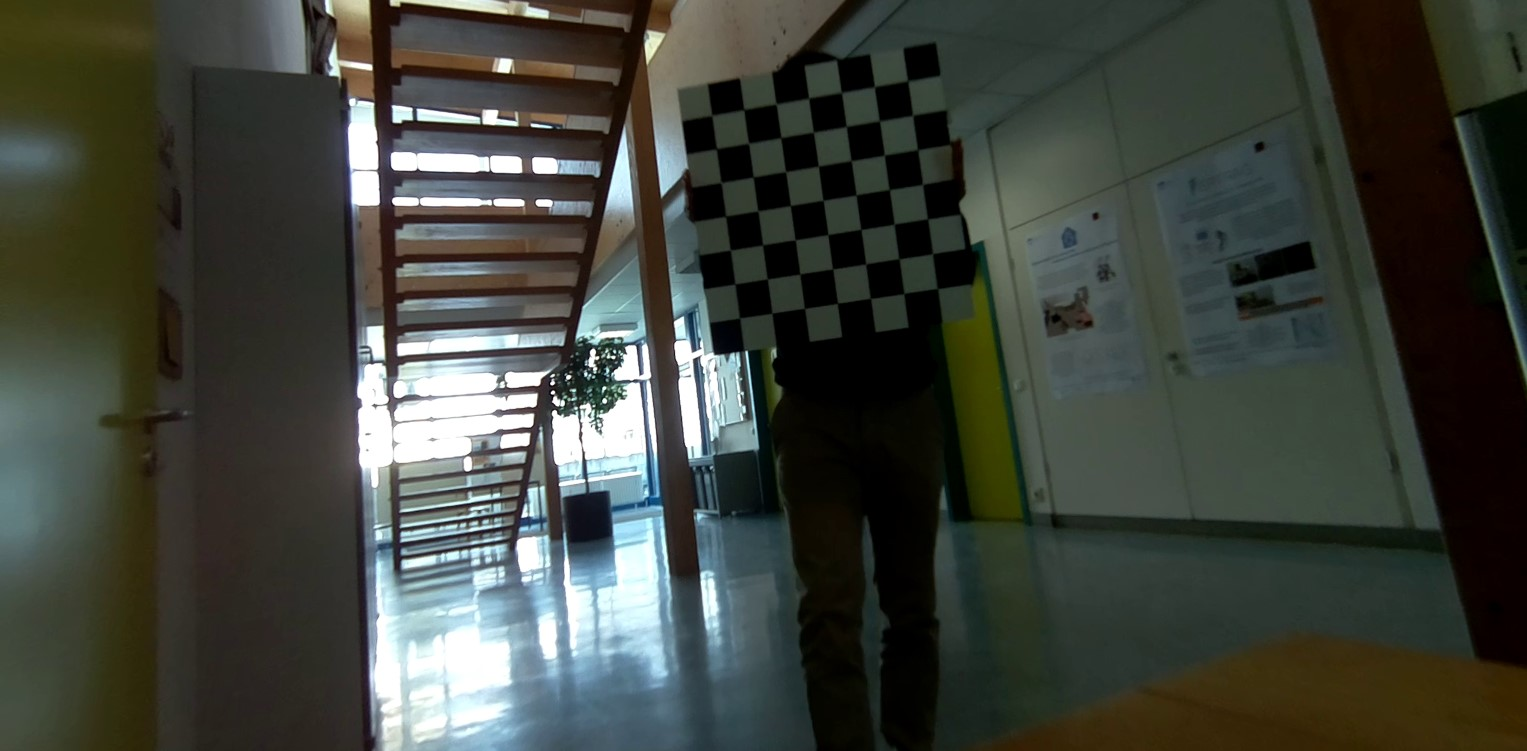
\includegraphics[width=\textwidth]{figures/addl/img13_5.jpg}
        \caption{Undistorted frame}
    \end{subfigure}
    \caption{Undistortion result of video 2 frame (3)}
    \label{fig:dist_2a3}
\end{figure}

\begin{figure}[h]
    \centering
    \begin{subfigure}[b]{0.48\textwidth}
        \centering
        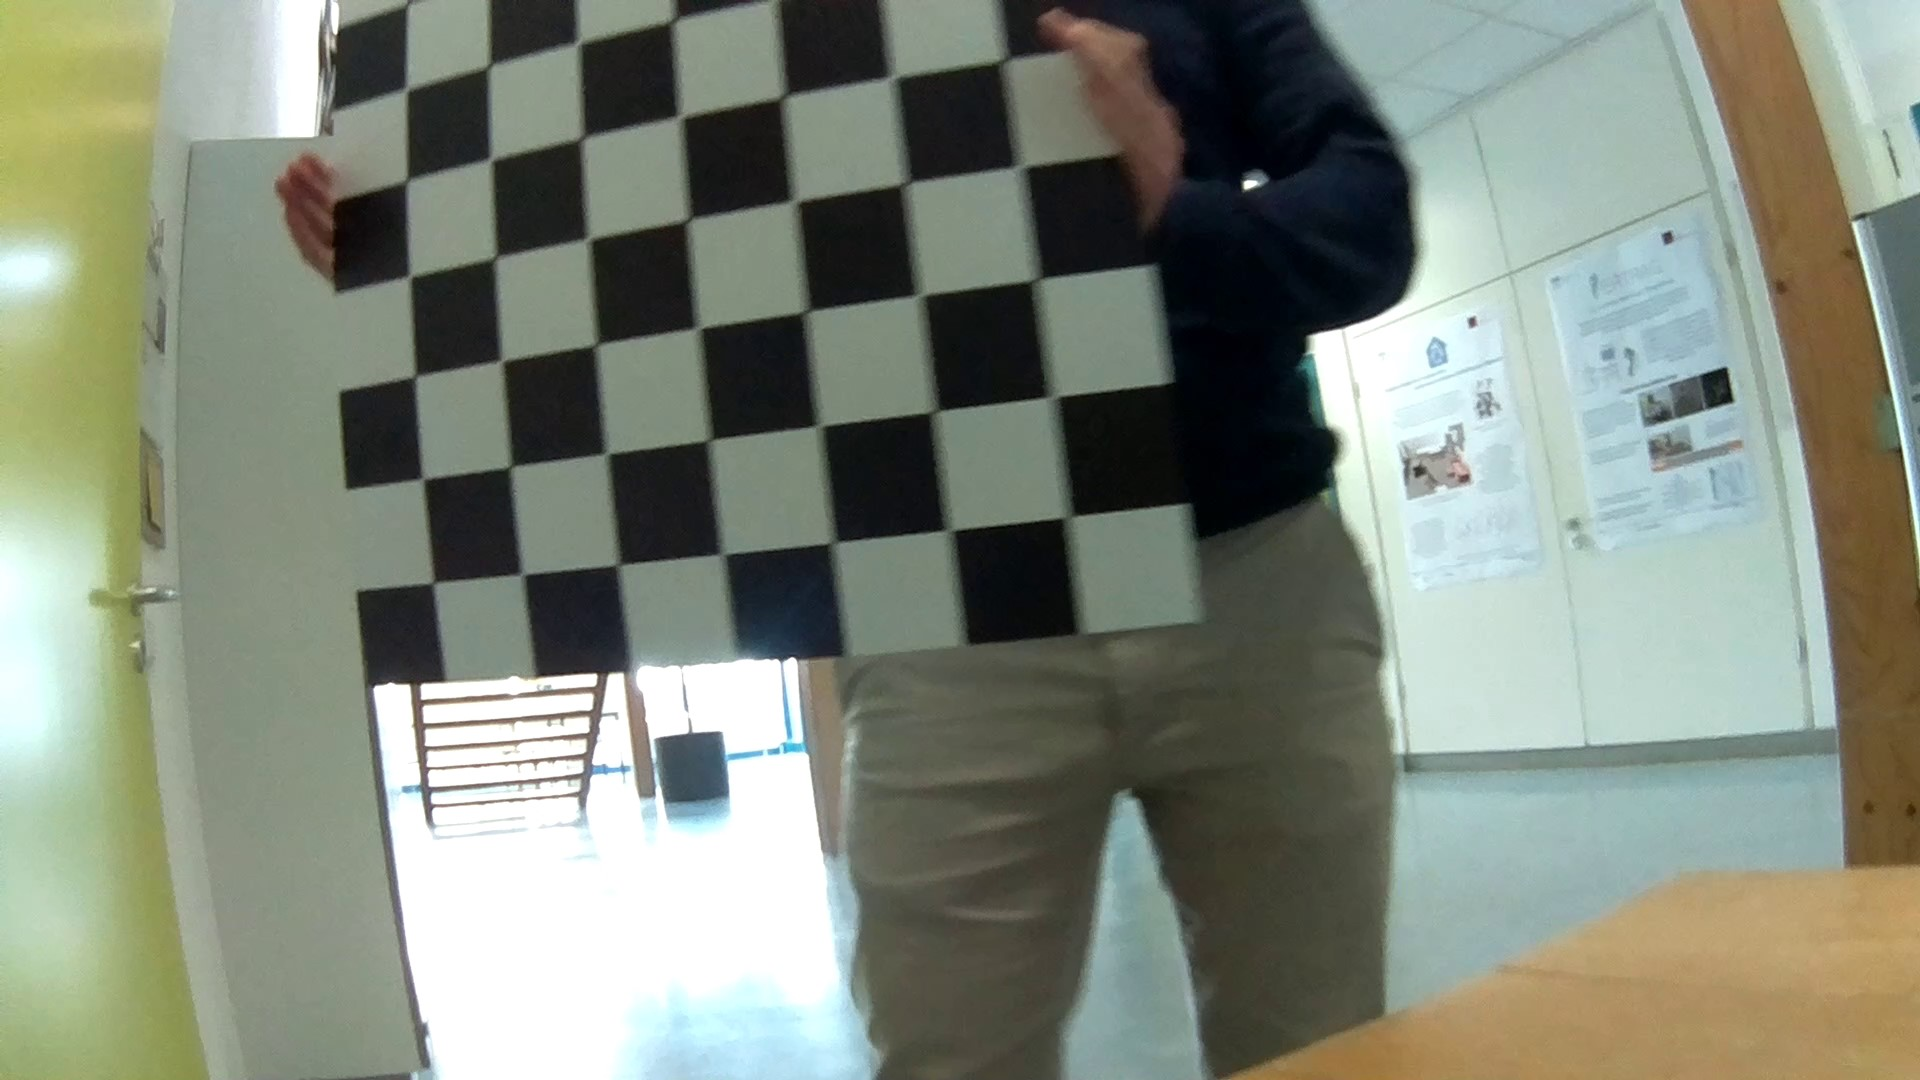
\includegraphics[width=\textwidth]{figures/addl/img14_0.jpg}
        \caption{Distorted frame}
    \end{subfigure}
    \hfill
    \begin{subfigure}[b]{0.48\textwidth}
        \centering
        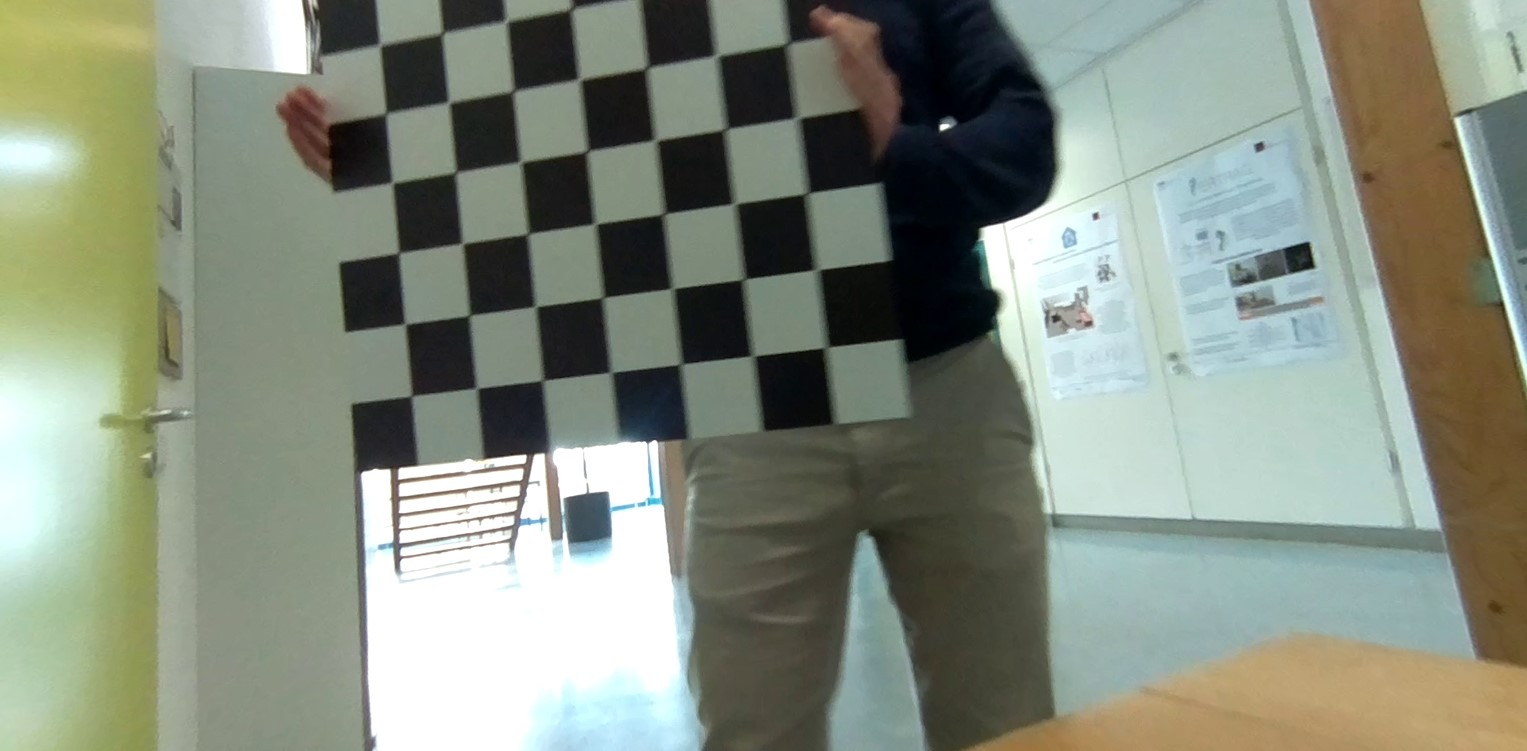
\includegraphics[width=\textwidth]{figures/addl/img14_5.jpg}
        \caption{Undistorted frame}
    \end{subfigure}
    \caption{Undistortion result of video 2 frame (4)}
    \label{fig:dist_2a4}
\end{figure}